\documentclass[11pt,a4paper]{article}

% Image mode: pdf.
% Image paths stay relative. In PDF mode, place same-basename PDF conversions
% of the chapter SVG files in the assets/ directory beside this source.

\usepackage{iftex}
\ifPDFTeX
  \PackageError{handout}{This template requires XeTeX or Tectonic}{Compile with xelatex or tectonic.}
\fi

\usepackage[a4paper,top=18mm,bottom=20mm,left=20mm,right=20mm,headsep=6mm]{geometry}
\usepackage{fontspec}
\usepackage{xeCJK}
\usepackage{amsmath}
\usepackage{unicode-math}

% Font settings are intentionally visible in the generated .tex file.
% These defaults target the macOS machine used for the released PDF.
% Change the family names when compiling on another system.
\setmainfont{Songti TC}
\setsansfont{Heiti TC}
\setmonofont{Menlo}
\setCJKmainfont{Songti TC}
\setCJKsansfont{Heiti TC}
\setCJKmonofont{Heiti TC}
\setmathfont{STIX Two Math}
\XeTeXlinebreaklocale "zh"
\XeTeXlinebreakskip=0pt plus 1pt

\usepackage{xcolor}
\definecolor{HandoutBlue}{HTML}{215A91}
\definecolor{HandoutBlueLight}{HTML}{EEF5FC}
\definecolor{HandoutGreen}{HTML}{39715A}
\definecolor{HandoutGreenLight}{HTML}{EFF8F3}
\definecolor{HandoutGold}{HTML}{8A641C}
\definecolor{HandoutGoldLight}{HTML}{FFF8E8}
\definecolor{HandoutInk}{HTML}{253142}
\definecolor{HandoutMuted}{HTML}{667085}

\usepackage{graphicx}
\makeatletter
% Pandoc 3 emits an accessibility `alt` key for raster/PDF images. Older
% graphicx releases do not know that key, so accept it without changing layout.
\@ifundefined{KV@Gin@alt}{\define@key{Gin}{alt}{}}{}
\newsavebox\pandoc@box
\newcommand*\pandocbounded[1]{%
  \sbox\pandoc@box{#1}%
  \Gscale@div\@tempa{\textheight}{\dimexpr\ht\pandoc@box+\dp\pandoc@box\relax}%
  \Gscale@div\@tempb{\linewidth}{\wd\pandoc@box}%
  \ifdim\@tempb\p@<\@tempa\p@\let\@tempa\@tempb\fi
  \ifdim\@tempa\p@<\p@\scalebox{\@tempa}{\usebox\pandoc@box}%
  \else\usebox{\pandoc@box}%
  \fi
}
\makeatother
\usepackage{float}
\floatplacement{figure}{H}
% Pandoc uses LTcaptype=none for uncaptioned longtables. The caption package
% expects that name to exist as a counter even though it is never displayed.
\newcounter{none}
\usepackage{caption}
\captionsetup[figure]{labelformat=empty,labelsep=none,font=small}

\usepackage{booktabs,longtable,array,calc}
\usepackage{etoolbox}
\makeatletter
\patchcmd\longtable{\par}{\if@noskipsec\mbox{}\fi\par}{}{}
\makeatother

\usepackage[most]{tcolorbox}
\tcbuselibrary{breakable,skins}
\newtcolorbox{HandoutLearningMap}{
  enhanced,breakable,colback=HandoutBlueLight,colframe=HandoutBlue,
  boxrule=0.8pt,arc=1.5mm,left=3mm,right=3mm,top=2mm,bottom=2mm,
  before skip=8pt,after skip=10pt
}
\newtcolorbox{HandoutWorkedExample}{
  enhanced,breakable,colback=HandoutGreenLight,colframe=HandoutGreen,
  boxrule=0.65pt,arc=1.5mm,left=3mm,right=3mm,top=2mm,bottom=2mm,
  before skip=8pt,after skip=10pt
}
\newtcolorbox{HandoutSelfCheck}{
  enhanced,breakable,colback=HandoutGoldLight,colframe=HandoutGold,
  boxrule=0.65pt,arc=1.5mm,left=3mm,right=3mm,top=2mm,bottom=2mm,
  before skip=8pt,after skip=10pt
}

\usepackage{titlesec}
\titleformat{\section}{\sffamily\bfseries\Large\color{HandoutBlue}}{}{0pt}{}
\titleformat{\subsection}{\sffamily\bfseries\large\color{HandoutInk}}{}{0pt}{}
\titleformat{\subsubsection}{\sffamily\bfseries\normalsize\color{HandoutInk}}{}{0pt}{}
\titlespacing*{\section}{0pt}{1.4em}{0.55em}
\titlespacing*{\subsection}{0pt}{1.15em}{0.45em}
\titlespacing*{\subsubsection}{0pt}{0.9em}{0.35em}
\setcounter{secnumdepth}{-\maxdimen}

\usepackage{hyperref}
\usepackage{bookmark}
\IfFileExists{xurl.sty}{\usepackage{xurl}}{}
\urlstyle{same}
\hypersetup{
  colorlinks=true,
  linkcolor=HandoutBlue,
  urlcolor=HandoutBlue,
  citecolor=HandoutBlue,
  pdftitle={選化V-1 有機化學},
  pdfsubject={化學},
  pdfcreator={Pandoc with the HighSchooContent LaTeX template}
}

\setlength{\parindent}{0pt}
\setlength{\parskip}{0.55em plus 0.15em minus 0.1em}
\setlength{\emergencystretch}{3em}
\setlength{\LTpre}{0.5em}
\setlength{\LTpost}{0.5em}
\renewcommand{\arraystretch}{1.18}
\providecommand{\tightlist}{%
  \setlength{\itemsep}{0pt}\setlength{\parskip}{0pt}}
\pagestyle{plain}


\begin{document}

\begin{tcolorbox}[
  enhanced,colback=white,colframe=HandoutBlue,boxrule=1.1pt,arc=2mm,
  borderline west={3pt}{0pt}{HandoutBlue},left=5mm,right=4mm,top=4mm,bottom=4mm
]
{\sffamily\small\bfseries\color{HandoutBlue}學生講義}\par
{\sffamily\bfseries\LARGE\color{HandoutInk}選化V-1 有機化學}\par
\vspace{0.35em}{\large 由分子結構、官能基與反應證據，預測有機物的性質、轉換與高分子用途}\par
\vspace{0.45em}{\small\color{HandoutMuted}%
科目：化學
\quad 課程：普通高中選修化學 V
\quad 版本：學生版｜核心＋理解
\quad 校訂：2026-08-29
}\par
\vspace{0.25em}{\small\color{HandoutMuted}範圍：現行選修化學 V 第一章主線；涵蓋結構與組成、異構物、官能基與命名、烴、含氧與含氮化合物、聚合反應、天然與人造聚合物，並納入官能基檢驗與阿司匹靈製備的證據鏈}\par
\end{tcolorbox}


有機化學的核心是「結構決定性質，反應改變結構」。同一分子式可對應多種原子連接方式，一個官能基的差異就可改變溶解度、沸點、酸鹼性與反應種類。這套模型用於藥物合成、食品成分、材料選擇、燃料分析、分離純化與廢塑膠管理。

\begin{HandoutLearningMap}

\subsection{本章問題與能力}\label{ux672cux7ae0ux554fux984cux8207ux80fdux529b}

\begin{enumerate}
\def\labelenumi{\arabic{enumi}.}
\tightlist
\item
  如何在分子式、實驗式、結構式與鍵線式之間轉換？
\item
  如何由元素分析、燃燒數據與分子量決定分子式？
\item
  如何以官能基、主鏈、位碼與取代基命名？
\item
  烷、烯、炔與芳香烴的結構如何決定取代、加成或氧化證據？
\item
  含氧與含氮官能基如何串成反應路線？
\item
  如何用溶解度、酸鹼與官能基反應分離或辨認未知物？
\item
  加成聚合與縮合聚合如何連結單體、重複單元與副產物？
\item
  天然與人造聚合物的鍵結、鏈段排列與組態如何影響功能與回收？
\end{enumerate}

\end{HandoutLearningMap}

\section{1. 有機化合物的結構與組成}\label{ux6709ux6a5fux5316ux5408ux7269ux7684ux7d50ux69cbux8207ux7d44ux6210}

\subsection{1.1 碳骨架與結構表示}\label{ux78b3ux9aa8ux67b6ux8207ux7d50ux69cbux8868ux793a}

有機化合物以含碳的共價骨架為主。高中化學沿用分類慣例，把 \(CO\)、\(CO_2\)、碳酸與碳酸鹽、碳酸氫鹽、碳化物及簡單氰化物等少數含碳物質歸在無機化合物。這項分類用於組織性質與反應；判斷時需同時看化學式與物質類別。

碳通常形成四個共價鍵，可互相連成直鏈、支鏈、環與網狀結構。在中性封閉殼層分子中，氫形成一鍵、氧常形成二鍵、氮常形成三鍵。這些價數規則可用來檢查結構有無漏鍵或多鍵。

{\def\LTcaptype{none} % do not increment counter
\begin{longtable}[]{@{}lll@{}}
\toprule\noalign{}
表示法 & 保留的資訊 & 典型用途 \\
\midrule\noalign{}
\endhead
\bottomrule\noalign{}
\endlastfoot
分子式 & 各元素原子數 & 組成、分子量、不飽和度 \\
實驗式 & 原子數最簡整數比 & 元素分析的第一步 \\
展開結構式 & 所有鍵結 & 檢查價數、追蹤斷鍵成鍵 \\
簡式結構式 & 官能基與碳鏈分組 & 書寫反應式 \\
鍵線式 & 碳骨架、多重鍵與異原子 & 快速比較複雜結構 \\
\end{longtable}
}

鍵線式的線端與折點各代表一個碳；連在碳上的氫依碳四價自動補足；O、N、Cl 等異原子與其氫必須寫出。

\begin{figure}
\centering
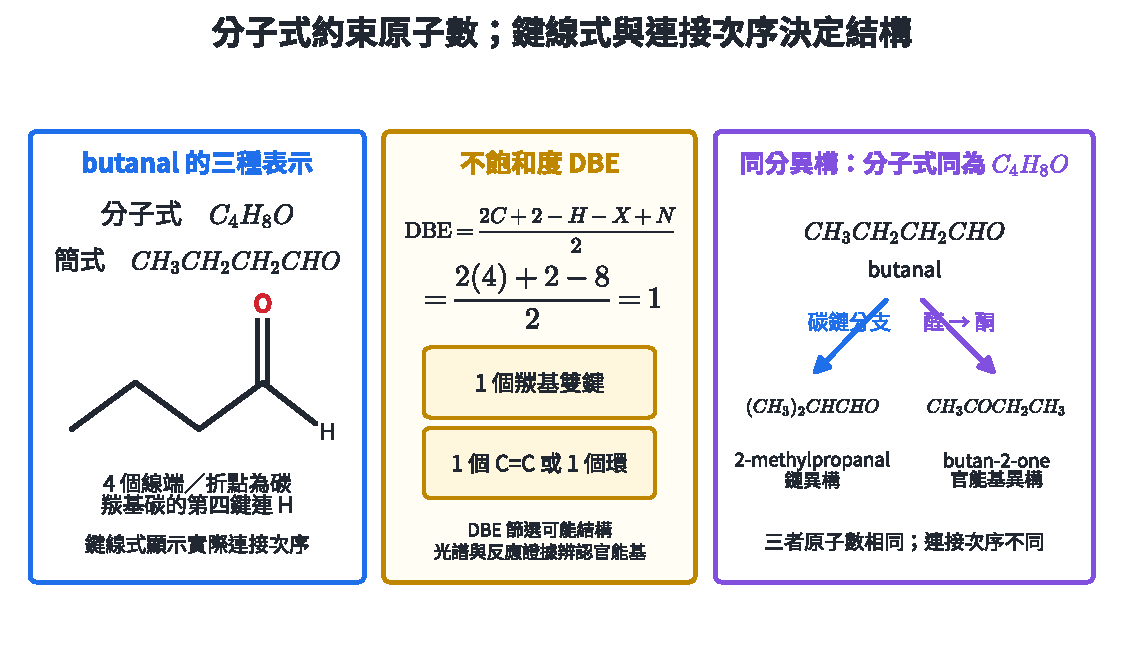
\includegraphics[width=0.98\linewidth,height=\textheight,keepaspectratio,alt={圖 1｜butanal 的分子式、簡式與鍵線式含相同原子；DBE 限制可能結構，分支與官能基改變則產生不同類型的同分異構物。}]{assets/選化V-1-結構表示與異構判斷.pdf}
\caption{圖 1｜butanal 的分子式、簡式與鍵線式含相同原子；DBE 限制可能結構，分支與官能基改變則產生不同類型的同分異構物。}
\end{figure}

\subsection{1.2 同分異構物}\label{ux540cux5206ux7570ux69cbux7269}

分子式相同而結構不同的化合物稱為\textbf{同分異構物}。本章的主要分類為：

\begin{itemize}
\tightlist
\item
  \textbf{鏈異構}：碳骨架不同，例如直鏈與支鏈。
\item
  \textbf{位置異構}：碳骨架相同，多重鍵或官能基位置不同。
\item
  \textbf{官能基異構}：分子式相同，官能基種類不同，例如醇與醚、醛與酮。
\item
  \textbf{順反異構}：鍵結次序相同，但限制旋轉使空間排列不同。烯類出現順反異構的必要條件是雙鍵上的每個碳都連著兩種不同取代基。
\end{itemize}

式量不足以辨認異構物，因為分子式相同。實際分析要結合沸點、光譜、化學檢驗或色層分析。

\subsection{1.3 不飽和度與組成分析}\label{ux4e0dux98fdux548cux5ea6ux8207ux7d44ux6210ux5206ux6790}

對中性、封閉殼層且只含 C、H、N、O、S 與鹵素 \(X\) 的分子，不飽和度（DBE）為

\[
\mathrm{DBE}=\frac{2C+2+N-H-X}{2}.
\]

一個環、一個雙鍵各貢獻 1，一個三鍵貢獻 2；O 與 S 不出現在式中。DBE 給出環與多重鍵的總數約束；唯一結構還需要官能基、光譜或物性證據。

完全燃燒中，樣品內的碳全進入 \(CO_2\)，氫全進入 \(H_2O\)：

\[
n(C)=n(CO_2),\qquad n(H)=2n(H_2O).
\]

若樣品只含 C、H、O，可以樣品質量扣除 C、H 質量求 O 質量。先求最簡整數比得實驗式，再以分子量決定倍數。

\begin{figure}
\centering
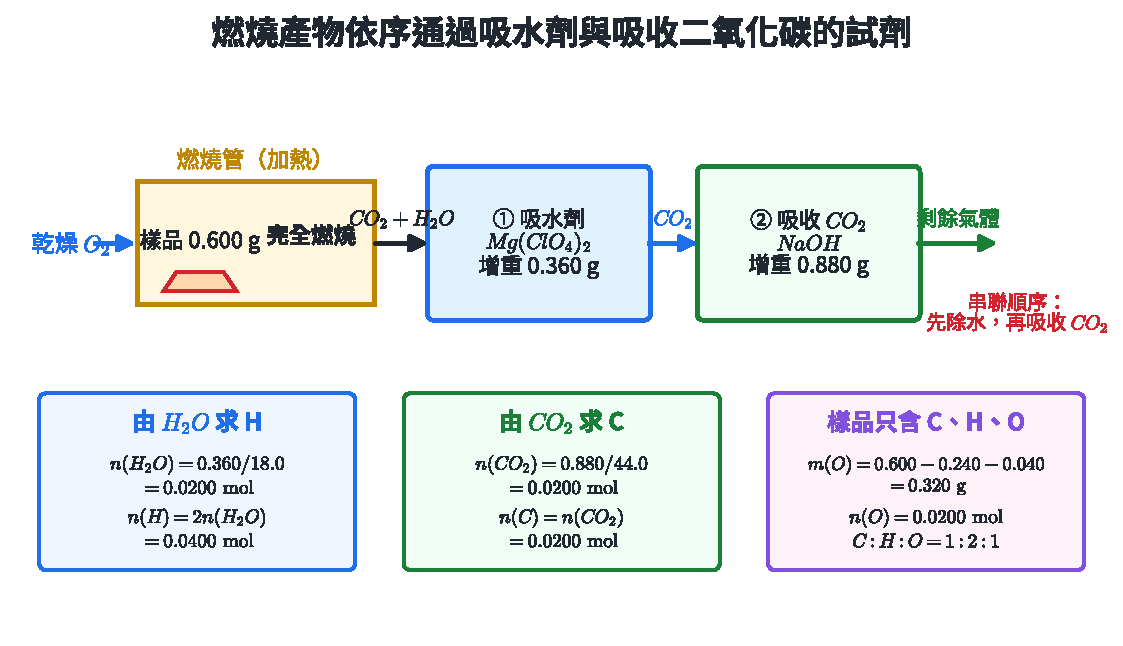
\includegraphics[width=0.98\linewidth,height=\textheight,keepaspectratio,alt={圖 2｜完全燃燒後的氣體先經吸水劑，再經二氧化碳吸收劑；兩瓶依序增重，才能分別換算 H 與 C 的物質的量。}]{assets/選化V-1-燃燒分析裝置與資料流.pdf}
\caption{圖 2｜完全燃燒後的氣體先經吸水劑，再經二氧化碳吸收劑；兩瓶依序增重，才能分別換算 H 與 C 的物質的量。}
\end{figure}

\begin{HandoutWorkedExample}

\subsection{示範 1｜分子式、DBE 與異構分類}\label{ux793aux7bc4-1ux5206ux5b50ux5f0fdbe-ux8207ux7570ux69cbux5206ux985e}

\(C_4H_8O\) 的 DBE 為

\[
\frac{2(4)+2-8}{2}=1.
\]

若指定分子含一個羧基且無環，該 DBE 已由 \(C=O\) 貢獻。符合條件的醛有 butanal 與 2-methylpropanal，屬鏈異構；酮有 butan-2-one。醛與酮之間屬官能基異構。三者皆符合同一分子式與 DBE，實驗上可再用銀鏡或斐林試驗辨認醛類。

\end{HandoutWorkedExample}

\begin{HandoutWorkedExample}

\subsection{示範 2｜由燃燒數據求分子式}\label{ux793aux7bc4-2ux7531ux71c3ux71d2ux6578ux64daux6c42ux5206ux5b50ux5f0f}

\(0.600\ \mathrm g\) 的 C、H、O 化合物完全燃燒，得 \(0.880\ \mathrm g\ CO_2\) 與 \(0.360\ \mathrm g\ H_2O\)；分子量為 \(60.0\) 。

\[
n(C)=\frac{0.880}{44.0}=0.0200\ \mathrm{mol},
\]

\[
n(H)=2\left(\frac{0.360}{18.0}\right)=0.0400\ \mathrm{mol}.
\]

C 與 H 的質量分別為 \(0.240\) g 與 \(0.0400\) g，因此

\[
m(O)=0.600-0.240-0.0400=0.320\ \mathrm g,
\qquad n(O)=\frac{0.320}{16.0}=0.0200\ \mathrm{mol}.
\]

原子比 \(C:H:O=1:2:1\)，實驗式為 \(CH_2O\)，實驗式量 \(30.0\)。分子量是其兩倍，故分子式為 \(C_2H_4O_2\)。依此資料仍無法區分乙酸與甲酸甲酯，還需酸鹼或光譜證據。

\end{HandoutWorkedExample}

\subsection{直接用途與適用邊界}\label{ux76f4ux63a5ux7528ux9014ux8207ux9069ux7528ux908aux754c}

\begin{itemize}
\tightlist
\item
  燃料與藥品品管以元素分析及分子量檢查組成；唯一結構還需光譜或化學反應。
\item
  DBE 適合快速篩掉不可能結構；離子、自由基或非典型價態需改用電子計數。
\item
  異構物的性質可不同，因此「同分子量」在藥物與溶劑辨認中不足以確認身分。
\end{itemize}

\subsection{練習 1}\label{ux7df4ux7fd2-1}

\begin{enumerate}
\def\labelenumi{\arabic{enumi}.}
\tightlist
\item
  求 \(C_6H_{10}O\) 的 DBE，並提出兩種可分配這些 DBE 的結構特徵組合。
\item
  判斷 pent-2-ene 是否可有順反異構，並以雙鍵兩碳的取代基說明。
\item
  一個鍵線式含六個折點與兩個線端，無環且只有單鍵。求其碳數與對應烷類分子式。
\item
  \(0.460\ \mathrm g\) 的 C、H、O 化合物完全燃燒，得 \(0.880\ \mathrm g\ CO_2\) 與 \(0.540\ \mathrm g\ H_2O\)。已知分子量為 \(46.0\)，求分子式。
\end{enumerate}

\subsection{練習 1 解析}\label{ux7df4ux7fd2-1-ux89e3ux6790}

\begin{enumerate}
\def\labelenumi{\arabic{enumi}.}
\tightlist
\item
  \(\mathrm{DBE}=[2(6)+2-10]/2=2\)。可由兩個雙鍵、一個三鍵、或一個環加一個雙鍵貢獻；氧不改變計算。
\item
  可以。第 2 號雙鍵碳連著 \(CH_3\) 與 H，第 3 號雙鍵碳連著 \(C_2H_5\) 與 H，兩端均有兩種取代基。
\item
  折點與線端各是一個碳，共 \(6+2=8\) 個碳。無環烷類通式 \(C_nH_{2n+2}\)，故為 \(C_8H_{18}\)。
\item
  \(n(C)=0.880/44.0=0.0200\) mol，\(n(H)=2(0.540/18.0)=0.0600\) mol。C、H 質量共 \(0.240+0.060=0.300\) g，故 \(m(O)=0.160\) g、\(n(O)=0.0100\) mol。比例 \(C:H:O=2:6:1\)，實驗式 \(C_2H_6O\) 的式量已為 \(46.0\)，所以分子式即 \(C_2H_6O\)。
\end{enumerate}

\section{2. 官能基與命名}\label{ux5b98ux80fdux57faux8207ux547dux540d}

\subsection{2.1 官能基是反應分類的單位}\label{ux5b98ux80fdux57faux662fux53cdux61c9ux5206ux985eux7684ux55aeux4f4d}

\textbf{官能基}是分子中主導典型化學性質的原子或原子團。碳骨架主要影響大小、形狀與分散力；官能基常決定極性、氫鍵、酸鹼性與反應位置。

{\def\LTcaptype{none} % do not increment counter
\begin{longtable}[]{@{}
  >{\raggedright\arraybackslash}p{(\linewidth - 6\tabcolsep) * \real{0.2500}}
  >{\raggedright\arraybackslash}p{(\linewidth - 6\tabcolsep) * \real{0.2500}}
  >{\raggedright\arraybackslash}p{(\linewidth - 6\tabcolsep) * \real{0.2500}}
  >{\raggedright\arraybackslash}p{(\linewidth - 6\tabcolsep) * \real{0.2500}}@{}}
\toprule\noalign{}
\begin{minipage}[b]{\linewidth}\raggedright
類別
\end{minipage} & \begin{minipage}[b]{\linewidth}\raggedright
特徵結構
\end{minipage} & \begin{minipage}[b]{\linewidth}\raggedright
命名詞尾／詞頭
\end{minipage} & \begin{minipage}[b]{\linewidth}\raggedright
主要證據或反應
\end{minipage} \\
\midrule\noalign{}
\endhead
\bottomrule\noalign{}
\endlastfoot
烯／炔 & \(C=C\) / \(C\equiv C\) & -ene / -yne & 加成、溴水與過錳酸鉀褪色 \\
醇 & \(R-OH\) & -ol／hydroxy- & 氫鍵、與 Na、氧化、脫水 \\
醚 & \(R-O-R'\) & alkoxy- & 極性但分子間無 \(O-H\) 氫鍵 \\
醛 & \(R-CHO\) & -al & 銀鏡、斐林／本尼迪克反應 \\
酮 & \(R-CO-R'\) & -one & 羧基；一般不呈上述醛類檢驗 \\
羧酸 & \(R-COOH\) & -oic acid & 弱酸，與 \(HCO_3^-\) 放 \(CO_2\) \\
酯 & \(R-COOR'\) & alkyl alkanoate & 酯化、水解、鹼性鹼化 \\
胺 & \(RNH_2,R_2NH,R_3N\) & -amine／amino- & 鹼性，成銔鹽 \\
醯胺 & \(R-CONH_2\) 等 & -amide & 強偶極、氫鍵、水解 \\
\end{longtable}
}

\begin{figure}
\centering
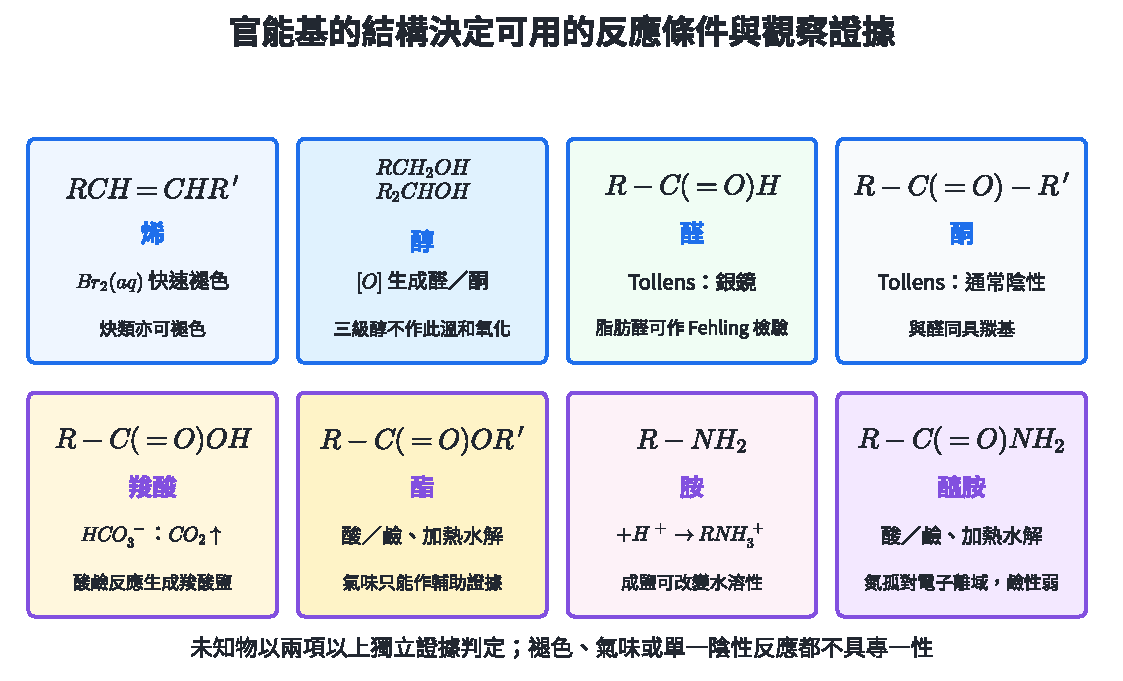
\includegraphics[width=0.99\linewidth,height=\textheight,keepaspectratio,alt={圖 3｜官能基圖譜以實際結構連到試劑條件、可觀察證據與適用限制；未知物需用兩項以上獨立證據判定。}]{assets/選化V-1-官能基分類圖譜.pdf}
\caption{圖 3｜官能基圖譜以實際結構連到試劑條件、可觀察證據與適用限制；未知物需用兩項以上獨立證據判定。}
\end{figure}

\subsection{2.2 系統命名的步驟}\label{ux7cfbux7d71ux547dux540dux7684ux6b65ux9a5f}

\begin{enumerate}
\def\labelenumi{\arabic{enumi}.}
\tightlist
\item
  依主要官能基選取包含它的最長碳鏈；它決定詞尾。
\item
  從使主要官能基位碼最小的一端編號；再比較多重鍵與取代基位碼。
\item
  辨認取代基的名稱、位碼與個數；重複取代基用 di-、tri- 等數目詞。
\item
  以字母順序排列不同取代基，組合「位碼---取代基---母體---主要詞尾」。
\item
  酯以連在氧上的烷基先命名，再寫羧酸端的 alkanoate；醚通常以較短端作 alkoxy 取代基。
\end{enumerate}

\begin{figure}
\centering
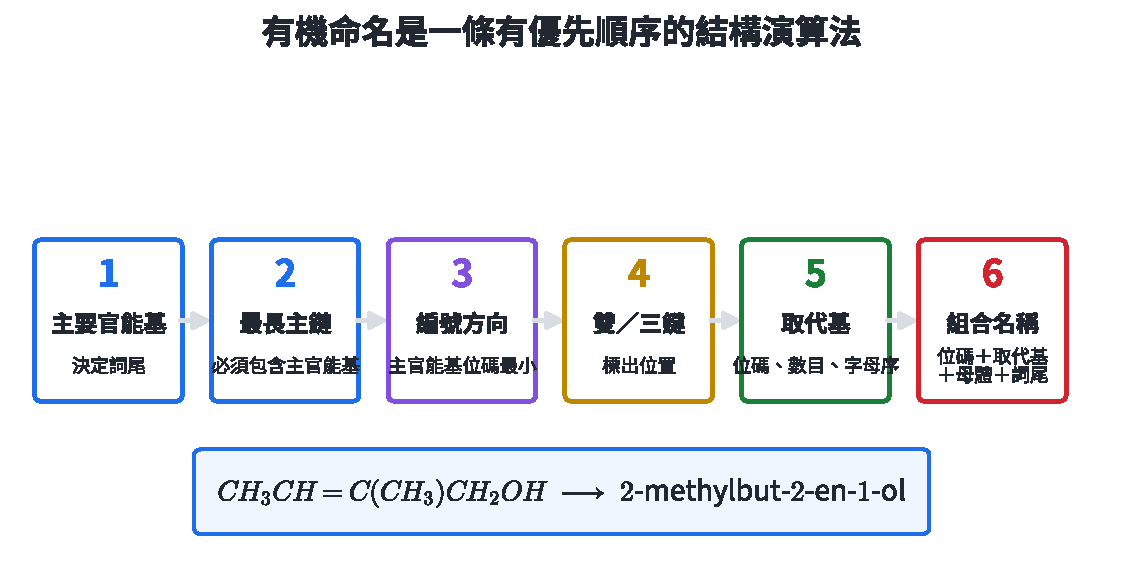
\includegraphics[width=0.98\linewidth,height=\textheight,keepaspectratio,alt={圖 4｜命名流程以主要官能基決定母體與編號，再將多重鍵、取代基與詞尾組合。}]{assets/選化V-1-有機命名流程.pdf}
\caption{圖 4｜命名流程以主要官能基決定母體與編號，再將多重鍵、取代基與詞尾組合。}
\end{figure}

\begin{HandoutWorkedExample}

\subsection{示範 3｜由結構數官能基與分子式}\label{ux793aux7bc4-3ux7531ux7d50ux69cbux6578ux5b98ux80fdux57faux8207ux5206ux5b50ux5f0f}

結構 \(HO-C_6H_4-COOCH_3\) 中，苯環直接連著 \(OH\)，所以該部分是酚；\(-COOCH_3\) 含羧酸衍生的 \(-COO-\)，是酯。原子數為

\[
C:6+1+1=8,\quad H:4+1+3=8,\quad O:1+2=3,
\]

故分子式為 \(C_8H_8O_3\)。苯環上的 \(OH\) 須分為酚，因為其酸鹼性與氧化反應不等同於脂肪族醇。

\end{HandoutWorkedExample}

\begin{HandoutWorkedExample}

\subsection{示範 4｜烯類命名與編號}\label{ux793aux7bc4-4ux70efux985eux547dux540dux8207ux7de8ux865f}

命名 \(CH_3CH_2C(CH_3)=CHCH_3\)。包含 \(C=C\) 的最長鏈有五個碳，由靠近雙鍵的右端編號，雙鍵位於 2，甲基位於 3，故名為 \textbf{3-methylpent-2-ene（3-甲基-2-戊烯）}。

若由左端編號，雙鍵位碼會成為 3；主鏈多重鍵優先取得較小位碼，因此選右端。

\end{HandoutWorkedExample}

\subsection{直接用途與適用邊界}\label{ux76f4ux63a5ux7528ux9014ux8207ux9069ux7528ux908aux754c-1}

\begin{itemize}
\tightlist
\item
  官能基表是實驗策略的索引：先由結構預測可觀察證據，再選擇檢驗，可減少無關的試藥。
\item
  藥品與聚合物規格需可唯一溝通的系統命名；商品名或俗名需搭配結構式才能作為結構證據。
\item
  命名次序取決於主要官能基優先權；本章使用課程常見類別，多官能基複雜優先權表不作額外背誦。
\end{itemize}

\subsection{練習 2}\label{ux7df4ux7fd2-2}

\begin{enumerate}
\def\labelenumi{\arabic{enumi}.}
\tightlist
\item
  對 \(CH_3CH_2CH_2OH\)、\(CH_3OCH_2CH_3\)、\(CH_3CH_2CHO\) 各指出官能基，並給出類別名稱。
\item
  命名 \(CH_3CH(CH_3)CH_2COOH\)。
\item
  寫出 ethyl ethanoate 的簡式結構式，並指出羧酸端與醇端的碳數。
\item
  一分子同時含 \(C=C\)、\(OH\) 與 \(COOH\)。說明選主鏈、編號與詞尾的順序。
\end{enumerate}

\subsection{練習 2 解析}\label{ux7df4ux7fd2-2-ux89e3ux6790}

\begin{enumerate}
\def\labelenumi{\arabic{enumi}.}
\tightlist
\item
  \(CH_3CH_2CH_2OH\) 含羥基，屬醇；\(CH_3OCH_2CH_3\) 含 \(C-O-C\)，屬醚；\(CH_3CH_2CHO\) 含末端 \(-CHO\)，屬醛。
\item
  羧基碳編為 1，最長鏈四碳，甲基在 3，故為 \textbf{3-methylbutanoic acid（3-甲基丁酸）}。
\item
  ethyl ethanoate 為 \(CH_3COOCH_2CH_3\)。\(CH_3CO-\) 的羧酸端有二碳，\(-CH_2CH_3\) 的醇端也有二碳。
\item
  選擇同時包含 \(COOH\) 與 \(C=C\) 的最長鏈；羧基碳為 1；先定雙鍵位碼，\(OH\) 作 hydroxy- 取代基，名稱以 -oic acid 結尾。
\end{enumerate}

\section{3. 烴}\label{ux70f4}

\subsection{3.1 分類、結構與反應模型}\label{ux5206ux985eux7d50ux69cbux8207ux53cdux61c9ux6a21ux578b}

只含碳、氫的有機化合物稱為\textbf{烴}。非環狀的主要通式為：

\[
\text{烷類 }C_nH_{2n+2},\qquad
\text{單烯類 }C_nH_{2n},\qquad
\text{單炔類 }C_nH_{2n-2}.
\]

只含碳---碳單鍵的烴稱為\textbf{飽和烴}；含碳---碳雙鍵或三鍵的烴稱為\textbf{不飽和烴}。脂肪族烴包含鏈狀與非芳香環狀骨架；芳香烴則含具離域 \(\pi\) 電子的芳香環。環本身也使分子式少兩個 H，因此通式需和 DBE 一起判讀。

烷類只含 \(\sigma\) 鍵，常見反應是燃燒與光照下的鹵化取代。烯、炔的 \(\pi\) 鍵電子較易參與反應，常見反應是加成：

\[
C=C+X-Y\longrightarrow -C(X)-C(Y)-.
\]

不對稱烯類與 \(HX\) 加成時，在課程常見條件下以 Markovnikov 方向為主：H 加到原先 H 較多的雙鍵碳，X 加到取代較多的碳。這是主產物預測；反應條件與機構改變時可出現不同選擇性。

苯環的六個 \(\pi\) 電子離域化，使芳香性骨架具特別穩定性。苯常保留芳香性進行取代反應，如催化溴化；在室溫、無催化條件下，不呈現一般烯類的溴水快速加成。

\begin{figure}
\centering
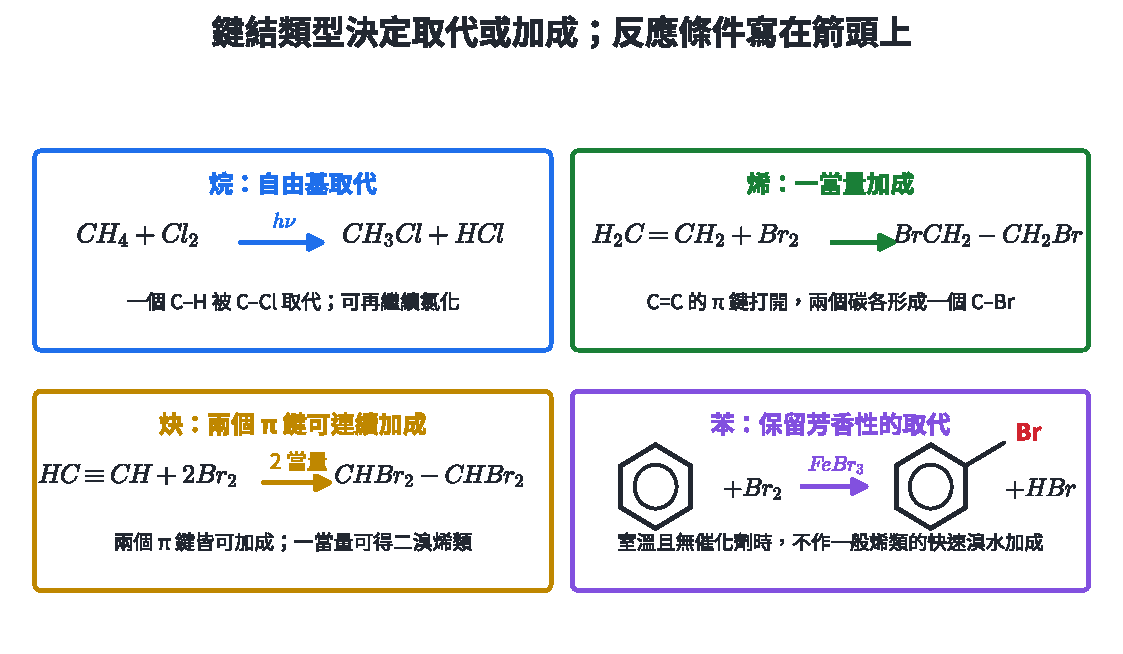
\includegraphics[width=0.99\linewidth,height=\textheight,keepaspectratio,alt={圖 5｜甲烷氯化為取代；乙烯與乙炔使 π 鍵加成；苯在 FeBr\_3 催化下取代並保留芳香環。各式均守恆原子數。}]{assets/選化V-1-烴類反應路線.pdf}
\caption{圖 5｜甲烷氯化為取代；乙烯與乙炔使 π 鍵加成；苯在 \(FeBr_3\) 催化下取代並保留芳香環。各式均守恆原子數。}
\end{figure}

\subsection{3.2 官能基證據與實驗安全}\label{ux5b98ux80fdux57faux8b49ux64daux8207ux5be6ux9a57ux5b89ux5168}

\begin{itemize}
\tightlist
\item
  \textbf{溴水}：烯或炔使棕紅色溴被消耗，溶液褪色；需有空白組並避開強光，因為其他還原性物質也可消耗溴。
\item
  \textbf{稀冷鹼性 \(KMnO_4\)}：雙鍵可被氧化，紫色減退並常見褐色 \(MnO_2\)；褪色只是化學證據，需搭配其他檢驗判斷結構。
\item
  \textbf{燃燒}：高碳氫比、混合不良時較易生成炭煙與 CO。通風與充足氧氣使燃燒較完全。
\end{itemize}

乙炔實驗中，氣體在集氣瓶內先和溴水或 \(KMnO_4\) 接觸，再依顏色與沉澱記錄。試管級實驗需戴護目鏡與手套、在通風處操作；溴與過錳酸鉀廢液依含氧化劑廢液收集，不直接倒入水槽。

\begin{HandoutWorkedExample}

\subsection{示範 5｜propene 的四種加成}\label{ux793aux7bc4-5propene-ux7684ux56dbux7a2eux52a0ux6210}

對 \(CH_3CH=CH_2\)：

\begin{enumerate}
\def\labelenumi{\arabic{enumi}.}
\tightlist
\item
  \(+H_2/Ni\) 斷開 \(\pi\) 鍵並在兩碳各加 H，得 \(CH_3CH_2CH_3\)。
\item
  \(+Br_2\) 在兩碳各加 Br，得 \(CH_3CHBrCH_2Br\)。
\item
  \(+HCl\) 主產物按 Markovnikov 方向，得 \(CH_3CHClCH_3\)。
\item
  \(+H_2O/H^+\) 主產物為 \(CH_3CHOHCH_3\)。
\end{enumerate}

四種反應都使一個 \(C=C\) 轉成 \(C-C\)，所以每個分子各消耗一個小分子試劑。

\end{HandoutWorkedExample}

\begin{HandoutWorkedExample}

\subsection{示範 6｜以反應條件辨認三種無色液體}\label{ux793aux7bc4-6ux4ee5ux53cdux61c9ux689dux4ef6ux8fa8ux8a8dux4e09ux7a2eux7121ux8272ux6db2ux9ad4}

未知物為 cyclohexane、cyclohexene、benzene。先在避光且無催化條件下加溴水：立即褪色者為 cyclohexene，因其 \(C=C\) 進行加成。餘下兩者另取新樣品，加 \(Br_2/FeBr_3\)：反應並保留環骨架者為 benzene，屬芳香親電取代；cyclohexane 需光照自由基條件才明顯溴化。

檢驗必須分批使用新樣品，因為第一步加入的試劑會改變後續條件。

\end{HandoutWorkedExample}

\subsection{直接用途與適用邊界}\label{ux76f4ux63a5ux7528ux9014ux8207ux9069ux7528ux908aux754c-2}

\begin{itemize}
\tightlist
\item
  烯類加成是氫化油脂、溶劑合成與聚合的基礎；產物選擇還受催化劑、溶劑與機構影響。
\item
  烴類燃燒的熱值與污染排放直接關係燃料設計；黑煙只能作質性證據，無法獨立決定分子結構。
\item
  溴水與 \(KMnO_4\) 檢驗能證明樣品發生了反應；還原性雜質也可使它們褪色，因此需交叉證據。
\end{itemize}

\subsection{練習 3}\label{ux7df4ux7fd2-3}

\begin{enumerate}
\def\labelenumi{\arabic{enumi}.}
\tightlist
\item
  寫出 1 mol ethyne 分別完全加成 \(H_2\) 與 \(Br_2\) 所需的最大莫耳數，並寫出產物。
\item
  預測 2-methylpropene 與 HCl 的主產物，並說明 H 與 Cl 的加成位置。
\item
  比較 benzene 與 cyclohexene 在「\(Br_2\)、室溫、無催化」條件下的觀察，以鍵結解釋。
\item
  某烴 \(0.100\) mol 完全燃燒生成 \(0.400\) mol \(CO_2\) 與 \(0.500\) mol \(H_2O\)。求分子式並分類。
\end{enumerate}

\subsection{練習 3 解析}\label{ux7df4ux7fd2-3-ux89e3ux6790}

\begin{enumerate}
\def\labelenumi{\arabic{enumi}.}
\tightlist
\item
  一個 \(C\equiv C\) 含兩個 \(\pi\) 鍵，1 mol ethyne 最多加 2 mol \(H_2\) 得 ethane，或加 2 mol \(Br_2\) 得 \(CHBr_2CHBr_2\)。
\item
  \(CH_2=C(CH_3)_2\) 中，H 加在原先 H 較多的末端 \(CH_2\)，Cl 加在中央碳，主產物為 2-chloro-2-methylpropane。
\item
  cyclohexene 的局部 \(C=C\) 可加成而使溴水快速褪色；benzene 的 \(\pi\) 電子離域化，在這些條件下溴水顏色保留。
\item
  每 mol 烴生 4 mol \(CO_2\) 與 5 mol \(H_2O\)，故分子式 \(C_4H_{10}\)，符合 \(C_nH_{2n+2}\)，是烷類。
\end{enumerate}

\section{4. 醇、醚及酚}\label{ux9187ux919aux53caux915a}

\subsection{4.1 結構、分子間作用力與溶解度}\label{ux7d50ux69cbux5206ux5b50ux9593ux4f5cux7528ux529bux8207ux6eb6ux89e3ux5ea6}

醇的羥基連在飽和碳上，酚的羥基直接連在苯環上，醚則為 \(R-O-R'\)。醇與酚可以 \(O-H\) 同時當氫鍵供體與受體，醚只能用氧上孤對電子當受體。對分子量接近的化合物，醇的沸點通常高於醚與烷類。

碳鏈增長時，非極性部分比例上升，低級醇的水溶性因此逐漸降低。這是「羥基與水的氫鍵」和「碳氫骨架疏水性」競爭的結果。

\begin{figure}
\centering
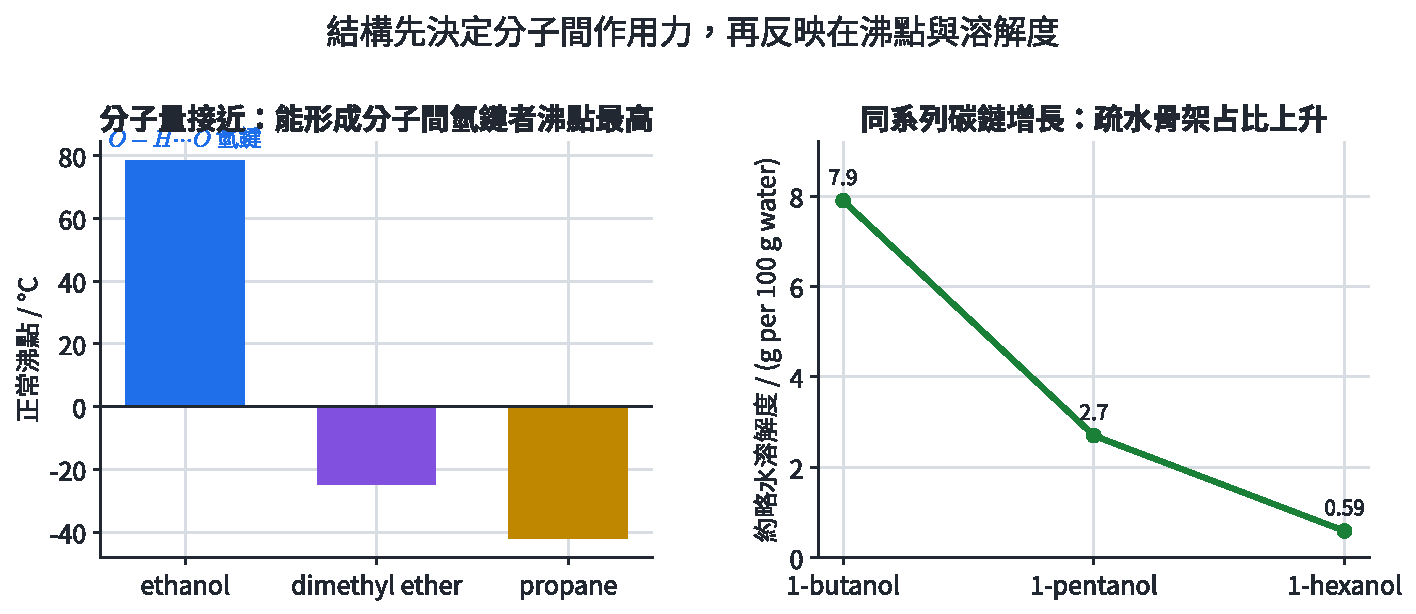
\includegraphics[width=0.98\linewidth,height=\textheight,keepaspectratio,alt={圖 6｜分子量接近時，可形成分子間 O-H\textbackslash cdots O 氫鍵的醇具較高沸點；碳鏈增長則降低水溶性。}]{assets/選化V-1-分子間作用力與沸點.pdf}
\caption{圖 6｜分子量接近時，可形成分子間 \(O-H\cdots O\) 氫鍵的醇具較高沸點；碳鏈增長則降低水溶性。}
\end{figure}

\subsection{4.2 醇的反應與酚的證據}\label{ux9187ux7684ux53cdux61c9ux8207ux915aux7684ux8b49ux64da}

一級醇、二級醇依羥基所連碳上的碳取代基數分類。溫和氧化的鍵結條件是羥基碳上存在 H：

\[
\text{一級醇}\rightarrow\text{醛}\rightarrow\text{羧酸},
\qquad
\text{二級醇}\rightarrow\text{酮}.
\]

三級醇的羥基碳無 H，因此不符合這條不斷碳---碳鍵的溫和氧化路徑。醇還可以：

\[
2ROH+2Na\rightarrow2RONa+H_2,
\]

\[
\text{醇}\xrightarrow[\text{加熱}]{\text{濃酸}}\text{烯}+H_2O.
\]

酚比脂肪族醇酸性強，可與強鹼形成酚鹽；部分酚類與 \(Fe^{3+}\) 形成有色錯合物，可作檢驗證據。

\begin{figure}
\centering
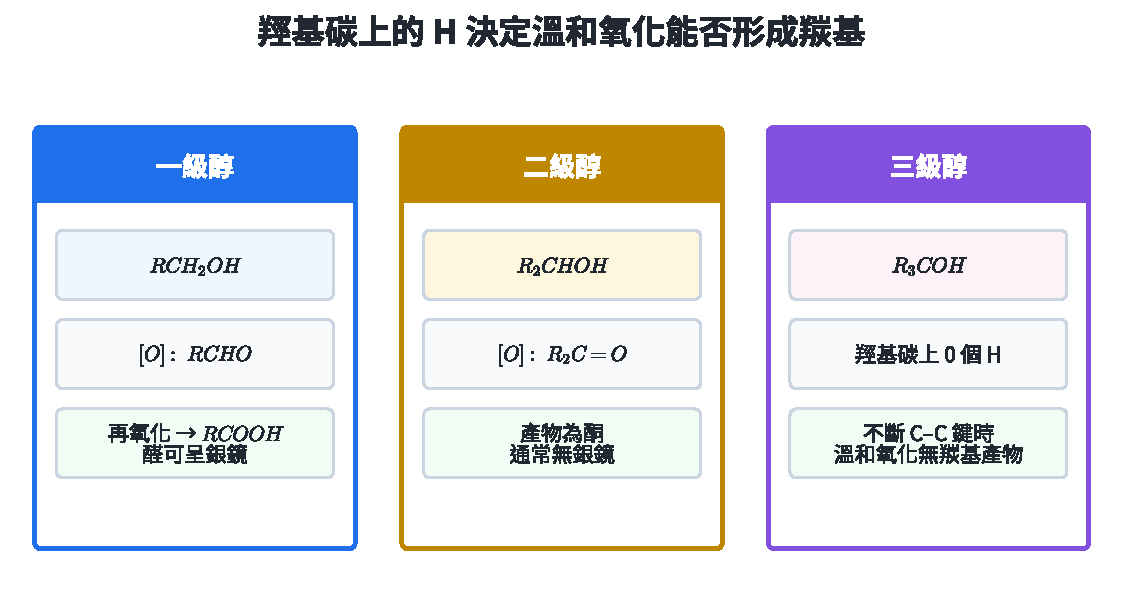
\includegraphics[width=0.98\linewidth,height=\textheight,keepaspectratio,alt={圖 7｜先依羥基碳的取代模式分類，再由產物的羰基位置與化學檢驗判斷氧化路線。}]{assets/選化V-1-醇氧化與官能基檢驗.pdf}
\caption{圖 7｜先依羥基碳的取代模式分類，再由產物的羰基位置與化學檢驗判斷氧化路線。}
\end{figure}

\begin{HandoutWorkedExample}

\subsection{示範 7｜由醇的類別預測氧化產物}\label{ux793aux7bc4-7ux7531ux9187ux7684ux985eux5225ux9810ux6e2cux6c27ux5316ux7522ux7269}

比較 butan-1-ol、butan-2-ol 與 2-methylpropan-2-ol。

\begin{itemize}
\tightlist
\item
  butan-1-ol 的羥基碳連一個碳，是一級醇；溫和氧化先得 butanal，繼續氧化得 butanoic acid。
\item
  butan-2-ol 的羥基碳連兩個碳，是二級醇；氧化得 butan-2-one。
\item
  2-methylpropan-2-ol 的羥基碳連三個碳且無 H，溫和氧化無對應羰基產物。
\end{itemize}

轉換前後碳骨架保持不變，是檢查產物的第一個條件。

\end{HandoutWorkedExample}

\begin{HandoutWorkedExample}

\subsection{示範 8｜由沸點與氧化證據辨認異構物}\label{ux793aux7bc4-8ux7531ux6cb8ux9edeux8207ux6c27ux5316ux8b49ux64daux8fa8ux8a8dux7570ux69cbux7269}

三種 \(C_3H_8O\) 樣品 A、B、C 的資料為：A 沸點 \(97^\circ\mathrm C\)，氧化後呈銀鏡；B 沸點 \(82^\circ\mathrm C\)，氧化後不呈銀鏡；C 沸點 \(-25^\circ\mathrm C\)，在同條件下無明顯氧化。

A、B 高沸點表示可形成分子間氫鍵，是醇；A 生成能呈銀鏡的醛，故 A 為 propan-1-ol。B 生成不呈銀鏡的酮，故 B 為 propan-2-ol。C 沸點大幅較低且不參與醇的氧化路徑，為 methoxyethane。判斷同時用到物理與化學證據。

\end{HandoutWorkedExample}

\subsection{直接用途與適用邊界}\label{ux76f4ux63a5ux7528ux9014ux8207ux9069ux7528ux908aux754c-3}

\begin{itemize}
\tightlist
\item
  溶劑選擇可用極性、氫鍵與碳鏈長度估計互溶性；精密溶解度還需溫度與實測數據。
\item
  酒精呼氣或製程檢測利用醇氧化與氧化劑顏色變化；顏色反應需有校正曲線才能定量。
\item
  酚性羥基影響藥物、色素與抗氧化物的酸鹼與反應；\(FeCl_3\) 顯色不具對所有酚的唯一性。
\end{itemize}

\subsection{練習 4}\label{ux7df4ux7fd2-4}

\begin{enumerate}
\def\labelenumi{\arabic{enumi}.}
\tightlist
\item
  將 ethanol、dimethyl ether、propane 依預期沸點由高至低排序，並指出主要分子間作用力。
\item
  寫出 3-methylbutan-1-ol 溫和氧化的第一個有機產物。
\item
  某 \(C_4H_{10}O\) 異構物可被氧化成酮。說明原醇的結構條件，並寫出一個符合的結構。
\item
  設計一個以氧化及銀鏡試驗區分 propan-1-ol 與 propan-2-ol 的步驟，寫出觀察鏈。
\end{enumerate}

\subsection{練習 4 解析}\label{ux7df4ux7fd2-4-ux89e3ux6790}

\begin{enumerate}
\def\labelenumi{\arabic{enumi}.}
\tightlist
\item
  ethanol \(>\) dimethyl ether \(>\) propane。ethanol 有分子間氫鍵、雙極力與分散力；dimethyl ether 有雙極力與分散力；propane 主要為分散力。
\item
  一級醇第一步得醛，產物為 3-methylbutanal：\((CH_3)_2CHCH_2CHO\)。
\item
  原醇必為二級醇，其羥基碳連兩個碳與一個 H。例如 butan-2-ol：\(CH_3CHOHCH_2CH_3\)，氧化得 butan-2-one。
\item
  分別將新樣品在同條件下溫和氧化，分離氧化產物後加 Tollens 試劑水浴加熱。propan-1-ol \(\rightarrow\) propanal，呈銀鏡；propan-2-ol \(\rightarrow\) propanone，無銀鏡。需設未反應試劑的空白組。
\end{enumerate}

\section{5. 醛、酮、羧酸及酯}\label{ux919bux916eux7fa7ux9178ux53caux916f}

\subsection{5.1 羰基的位置與檢驗}\label{ux7fb0ux57faux7684ux4f4dux7f6eux8207ux6aa2ux9a57}

醛的羰基在碳鏈末端，羰基碳連 H；酮的羰基碳連兩個碳基。兩者都具極性 \(C=O\)，但醛較易被氧化為羧酸，因此可以溫和氧化試劑區分：

\begin{itemize}
\tightlist
\item
  Tollens 試劑：醛還原 \(Ag^+\) 得銀鏡或銀黑沉積。
\item
  Fehling 或 Benedict 試劑：部分醛還原 \(Cu^{2+}\) 得磚紅 \(Cu_2O\)。
\end{itemize}

試驗結果與特定試劑、溫度及樣品結構有關；顏色或沉澱證據應搭配空白組與已知對照組。

Tollens 試劑現配現用，反應後立即依含銀廢液流程處理；存放或讓殘液乾涸可能形成對震動敏感的含銀物質，會直接改變實驗安全。

\subsection{5.2 羧酸、酯化與水解}\label{ux7fa7ux9178ux916fux5316ux8207ux6c34ux89e3}

羧酸在水中部分解離：

\[
RCOOH+H_2O\rightleftharpoons RCOO^-+H_3O^+.
\]

它可與碳酸氫鹽反應放出 \(CO_2\)，這是區分羧酸與一般醇、酚的常用證據。羧酸與醇在酸催化下建立酯化平衡：

\[
RCOOH+R'OH\rightleftharpoons RCOOR'+H_2O.
\]

增加一種反應物或移除水可使平衡偏向酯。酯在酸性水中可逆水解；在鹼性水溶液中得羧酸鹽與醇，又稱鹼化。油脂是甘油與高級脂肪酸的三酯，鹼化得甘油與脂肪酸鹽（肥皂）。

\begin{figure}
\centering
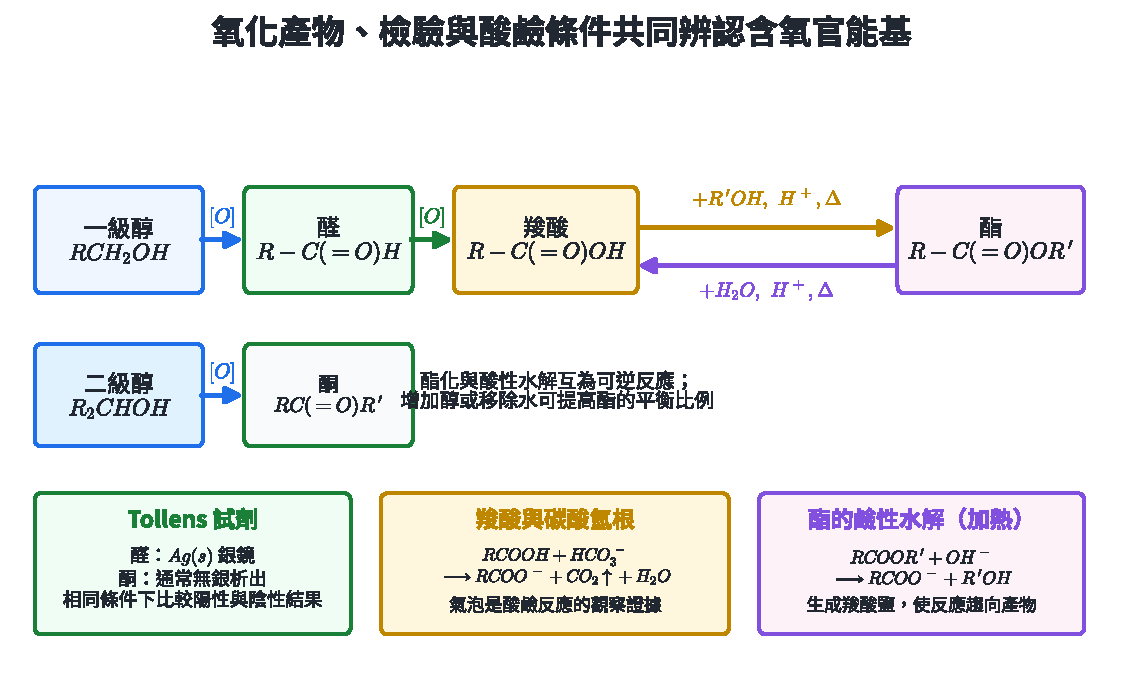
\includegraphics[width=0.99\linewidth,height=\textheight,keepaspectratio,alt={圖 8｜一、二級醇的氧化產物不同；銀鏡、碳酸氫根放氣、可逆酯化與鹼性水解各提供可列式的反應證據。}]{assets/選化V-1-羰基羧酸酯反應網.pdf}
\caption{圖 8｜一、二級醇的氧化產物不同；銀鏡、碳酸氫根放氣、可逆酯化與鹼性水解各提供可列式的反應證據。}
\end{figure}

\subsection{5.3 阿司匹靈製備的證據鏈}\label{ux963fux53f8ux5339ux9748ux88fdux5099ux7684ux8b49ux64daux93c8}

水楊酸與醋酸酐在酸催化下反應：

\[
\text{水楊酸}+\text{醋酸酐}
\longrightarrow
\text{乙醯水楊酸（阿司匹靈）}+\text{醋酸}.
\]

水楊酸的酚性 \(OH\) 轉成酯，羧基保留。實驗的連續證據為：加熱促進反應 → 加水消耗過量醋酸酐並冷卻結晶 → 減壓過濾 → 再結晶純化 → 乾燥後秤量求產率。\(FeCl_3\) 對未反應的酚性水楊酸常呈紫色，可作殘留反應物的質性證據；產物身分與純度還可用熔點區間等數據檢查。

醋酸酐具腐蝕與催淚風險，濃酸具腐蝕性；全程戴護目鏡、適用手套並在通風櫥操作。有機母液、酸性水相與固體殘渣依教室廢棄分類收集。

\begin{figure}
\centering
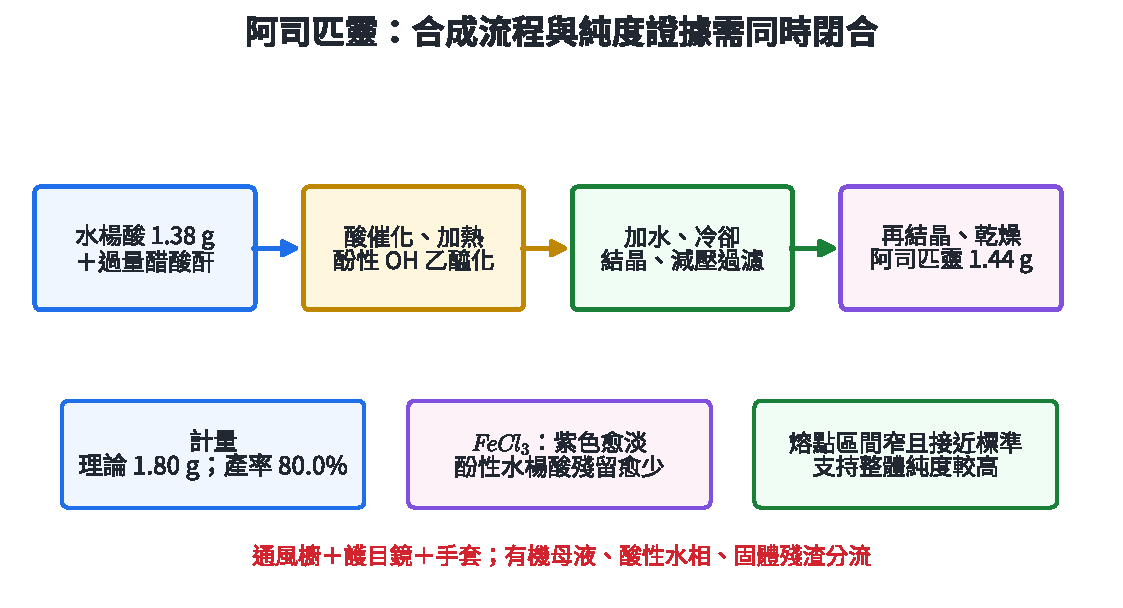
\includegraphics[width=0.99\linewidth,height=\textheight,keepaspectratio,alt={圖 9｜阿司匹靈實驗將反應、結晶、過濾、再結晶、產率與純度證據排成可檢查的資料流。}]{assets/選化V-1-阿司匹靈製備與純度.pdf}
\caption{圖 9｜阿司匹靈實驗將反應、結晶、過濾、再結晶、產率與純度證據排成可檢查的資料流。}
\end{figure}

\begin{HandoutWorkedExample}

\subsection{示範 9｜由三項檢驗辨認未知物}\label{ux793aux7bc4-9ux7531ux4e09ux9805ux6aa2ux9a57ux8fa8ux8a8dux672aux77e5ux7269}

未知水溶性樣品可能是 ethanal、propanone 或 ethanoic acid。對新樣品分批檢驗：

\begin{enumerate}
\def\labelenumi{\arabic{enumi}.}
\tightlist
\item
  加 \(NaHCO_3\) 有無色氣泡，且氣體使石灰水變濁，即有 \(CO_2\)，判為 ethanoic acid。
\item
  餘下者用 Tollens 試劑水浴加熱，生銀鏡者為 ethanal，因醛被氧化。
\item
  兩項均無上述證據者為 propanone。
\end{enumerate}

每步都設已知陽性對照與空白組，可區分「樣品無反應」與「試劑失效」。

\end{HandoutWorkedExample}

\begin{HandoutWorkedExample}

\subsection{示範 10｜阿司匹靈限量、產率與純度}\label{ux793aux7bc4-10ux963fux53f8ux5339ux9748ux9650ux91cfux7522ux7387ux8207ux7d14ux5ea6}

以 \(1.38\ \mathrm g\) 水楊酸（\(M=138\ \mathrm{g\,mol^{-1}}\)）和過量醋酸酐製備阿司匹靈（\(M=180\ \mathrm{g\,mol^{-1}}\)），乾燥得 \(1.44\ \mathrm g\) 結晶。

\[
n(\text{水楊酸})=\frac{1.38}{138}=0.0100\ \mathrm{mol}.
\]

反應係數為 \(1:1\)，理論阿司匹靈質量 \(=0.0100(180)=1.80\ \mathrm g\)，所以

\[
\text{產率}=\frac{1.44}{1.80}\times100\%=80.0\%.
\]

若產物遇 \(FeCl_3\) 呈明顯紫色，證據指向酚性水楊酸殘留；產率值本身只比較回收質量與理論質量，無法獨立證明純度。

\end{HandoutWorkedExample}

\subsection{直接用途與適用邊界}\label{ux76f4ux63a5ux7528ux9014ux8207ux9069ux7528ux908aux754c-4}

\begin{itemize}
\tightlist
\item
  銀鏡、還原糖與羧酸放氣試驗用於官能基篩檢；實際實驗室需以光譜、色層或多種對照完成確認。
\item
  酯化與水解用於香料、藥物、生質柴油與聚酯；平衡轉化率需同時考慮濃度、水與分離步驟。
\item
  阿司匹靈製備把化學計量、限量、純化與分析證據串在同一實驗；有結晶不等於已證明為純物質。
\end{itemize}

\subsection{練習 5}\label{ux7df4ux7fd2-5}

\begin{enumerate}
\def\labelenumi{\arabic{enumi}.}
\tightlist
\item
  寫出 propanal 與 propanone 在 Tollens 試驗的觀察差異，並指出被氧化的物質。
\item
  寫出 propanoic acid 與 ethanol 的酯化產物，並寫出一項提高平衡產率的操作。
\item
  \(0.200\) mol 甘油三酯完全鹼化，求甘油與脂肪酸鹽的莫耳數。
\item
  阿司匹靈再結晶後，收量由 \(1.50\) g 降為 \(1.20\) g，\(FeCl_3\) 呈色由深紫轉為極淡，熔點區間由 \(120\)--\(132^\circ\mathrm C\) 變為 \(134\)--\(136^\circ\mathrm C\)。分別說明收率與純度證據。
\end{enumerate}

\subsection{練習 5 解析}\label{ux7df4ux7fd2-5-ux89e3ux6790}

\begin{enumerate}
\def\labelenumi{\arabic{enumi}.}
\tightlist
\item
  propanal 是醛，還原 \(Ag^+\) 而呈銀鏡，自身被氧化成 propanoate（酸化後為 propanoic acid）；propanone 在這些條件下無銀鏡。
\item
  產物為 ethyl propanoate 與水：\(CH_3CH_2COOH+C_2H_5OH\rightleftharpoons CH_3CH_2COOC_2H_5+H_2O\)。可用過量一種反應物或連續移除水使平衡右移。
\item
  一個三酯水解得一個甘油與三個羧酸鹽，故得 \(0.200\) mol 甘油與 \(0.600\) mol 脂肪酸鹽。
\item
  再結晶損失部分產物，所以回收質量降低 \(0.30\) g。\(FeCl_3\) 呈色減弱表示酚性水楊酸殘留減少；熔點區間變窄且接近固定值，也支持純度提高。
\end{enumerate}

\section{6. 胺與醯胺}\label{ux80faux8207ux91afux80fa}

\subsection{6.1 胺的分類、鹼性與成鹽}\label{ux80faux7684ux5206ux985eux9e7cux6027ux8207ux6210ux9e7d}

胺可視為 \(NH_3\) 的一個、兩個或三個 H 被烴基取代，依氮上烴基數分為一級胺 \(RNH_2\)、二級胺 \(R_2NH\) 與三級胺 \(R_3N\)。氮的孤對電子可接受質子：

\[
RNH_2+H_2O\rightleftharpoons RNH_3^++OH^-,
\]

\[
RNH_2+HCl\rightarrow RNH_3^+Cl^-.
\]

中性胺常可溶於有機相；質子化後成為帶電銨鹽，水溶性通常顯著增加。這個可逆轉換是酸鹼萃取的基礎。胺的實際鹼性受取代基、溶劑與共振影響，因此只靠「幾級胺」不足以精確排序所有 \(K_b\)。

\subsection{6.2 醯胺的結構與水解}\label{ux91afux80faux7684ux7d50ux69cbux8207ux6c34ux89e3}

醯胺具有 \(-CONH_2\)、\(-CONHR\) 或 \(-CONR_2\)。氮的孤對電子和羰基共振，使 \(C-N\) 具有部分雙鍵性並降低氮接受質子的能力；醯胺的鹼性通常遠弱於胺。含 \(N-H\) 的一、二級醯胺可形成分子間氫鍵，常具有較高沸點或熔點。

醯胺在酸或鹼催化並加熱時可水解：

\[
RCONH_2+H_2O+H^+\xrightarrow{\Delta}RCOOH+NH_4^+,
\]

\[
RCONH_2+OH^-\xrightarrow{\Delta}RCOO^-+NH_3.
\]

酸性條件下胺端以銨離子存在；鹼性條件下羧酸端以羧酸根存在。蛋白質中的肽鍵就是醯胺鍵，其水解需適當催化與條件。

\begin{figure}
\centering
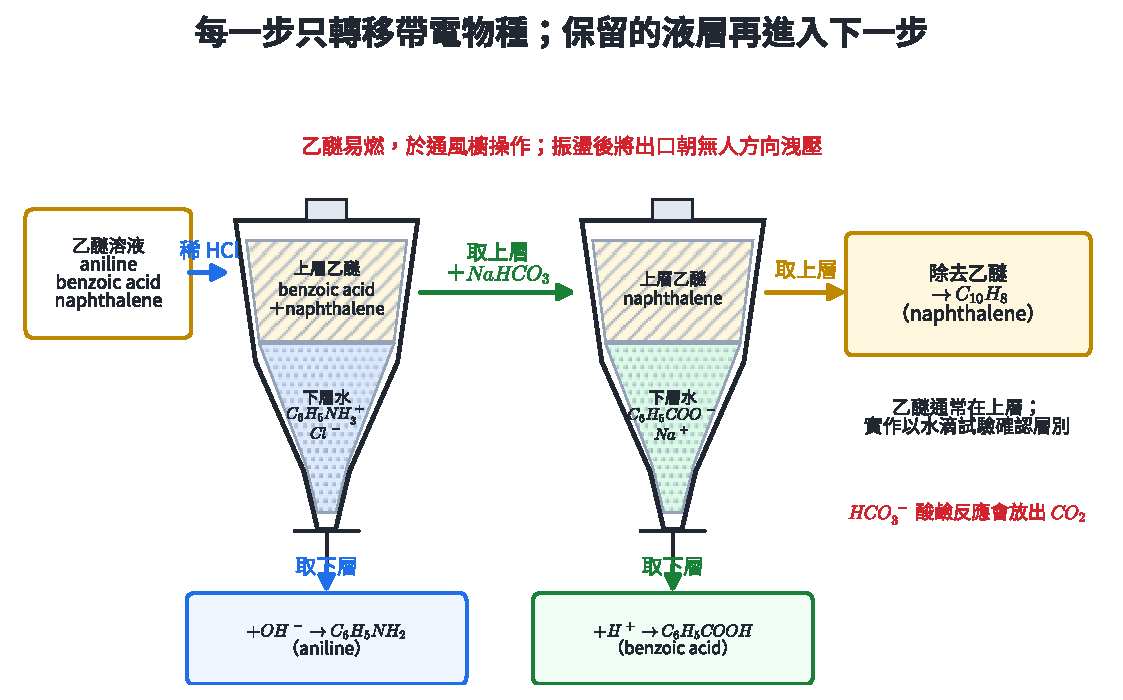
\includegraphics[width=0.99\linewidth,height=\textheight,keepaspectratio,alt={圖 10｜先以稀鹽酸把苯胺轉入水層，再以碳酸氫鈉把苯甲酸轉入水層；每一步明示保留哪一層及如何復原中性產物。}]{assets/選化V-1-酸鹼萃取流程.pdf}
\caption{圖 10｜先以稀鹽酸把苯胺轉入水層，再以碳酸氫鈉把苯甲酸轉入水層；每一步明示保留哪一層及如何復原中性產物。}
\end{figure}

\begin{HandoutWorkedExample}

\subsection{示範 11｜以酸鹼萃取分離苯胺與萘}\label{ux793aux7bc4-11ux4ee5ux9178ux9e7cux8403ux53d6ux5206ux96e2ux82efux80faux8207ux8418}

乙醚層含苯胺 \(C_6H_5NH_2\) 與中性萘。加入稀 HCl 並振盪、洩壓後，苯胺被質子化：

\[
C_6H_5NH_2+HCl\rightarrow C_6H_5NH_3^+Cl^-.
\]

苯胺鹽進入水層，萘留在乙醚層。分出水層，加 \(NaOH\) 至鹼性：

\[
C_6H_5NH_3^++OH^-\rightarrow C_6H_5NH_2+H_2O.
\]

中性苯胺重新析出或可再被有機溶劑萃取。分液漏斗振盪時有蒸氣壓與放氣風險，需朝無人方向頻繁洩壓；層位由密度資料或滴水測試確認。

\end{HandoutWorkedExample}

\begin{HandoutWorkedExample}

\subsection{示範 12｜醯胺分類與鹼性水解物種}\label{ux793aux7bc4-12ux91afux80faux5206ux985eux8207ux9e7cux6027ux6c34ux89e3ux7269ux7a2e}

\(CH_3CONHCH_3\) 中，氮連一個醯基、一個甲基與一個 H，屬二級醯胺，名稱可寫 N-methylethanamide。其鹼性水解為

\[
CH_3CONHCH_3+OH^-\xrightarrow{\Delta}CH_3COO^-+CH_3NH_2.
\]

產物的羧酸端是 ethanoate，因反應介質為鹼性；氮端形成 methylamine。原分子雖有一個 \(N-H\) 可作氫鍵供體，但氮孤對電子受羰基共振離域，鹼性低於 methylamine。

\end{HandoutWorkedExample}

\subsection{直接用途與適用邊界}\label{ux76f4ux63a5ux7528ux9014ux8207ux9069ux7528ux908aux754c-5}

\begin{itemize}
\tightlist
\item
  酸鹼萃取用於藥物、生物鹼與有機酸的分離；前提是目標物在所選 pH 能有效轉成帶電形態，且兩液相互不相溶。
\item
  胺形成水溶性鹽可改善部分藥物的製劑性質；體內吸收還受 pH、膜通透性與其他官能基影響。
\item
  醯胺鍵提供尼龍、蛋白質與多種藥物的結構；水解速度取決於催化、溫度與鄰近結構，反應式不代表室溫純水中迅速進行。
\end{itemize}

\subsection{練習 6}\label{ux7df4ux7fd2-6}

\begin{enumerate}
\def\labelenumi{\arabic{enumi}.}
\tightlist
\item
  將 \(CH_3NH_2\)、\((CH_3)_2NH\)、\((CH_3)_3N\) 依氮上烴基數分類，並寫出各自與 HCl 反應後的離子。
\item
  說明 acetamide 的沸點為何高於分子量接近且無氫鍵的化合物，並指出供體與受體。
\item
  乙醚中含 benzoic acid 與 naphthalene。寫出用 \(NaHCO_3\) 分離的反應、各層物種與回收 benzoic acid 的操作。
\item
  寫出 propanamide 在酸性水解與鹼性水解後的主要含碳產物及含氮物種。
\end{enumerate}

\subsection{練習 6 解析}\label{ux7df4ux7fd2-6-ux89e3ux6790}

\begin{enumerate}
\def\labelenumi{\arabic{enumi}.}
\tightlist
\item
  \(CH_3NH_2\)、\((CH_3)_2NH\)、\((CH_3)_3N\) 分別是一、二、三級胺；與 HCl 後分別為 \(CH_3NH_3^+\)、\((CH_3)_2NH_2^+\)、\((CH_3)_3NH^+\)，並有 \(Cl^-\) 作反離子。
\item
  acetamide 的 \(N-H\) 可作氫鍵供體，羰基氧可作氫鍵受體，分子間吸引較強，汽化需較多能量。氮孤對電子主要參與共振，羰基氧是主要受體。
\item
  \(C_6H_5COOH+HCO_3^-\rightarrow C_6H_5COO^-+CO_2+H_2O\)。benzoate 進水層，中性 naphthalene 留乙醚層；分出水層後加酸至酸性，使 \(C_6H_5COOH\) 析出，再過濾。
\item
  酸性水解得 propanoic acid 與 \(NH_4^+\)；鹼性水解得 propanoate 與 \(NH_3\)。介質決定酸、鹼產物的主要質子化形態。
\end{enumerate}

\section{7. 聚合物與聚合反應}\label{ux805aux5408ux7269ux8207ux805aux5408ux53cdux61c9}

\subsection{7.1 單體、重複單元與聚合度}\label{ux55aeux9ad4ux91cdux8907ux55aeux5143ux8207ux805aux5408ux5ea6}

\textbf{聚合物}是許多重複結構單元以共價鍵連成的高分子；形成聚合物的小分子稱\textbf{單體}。若聚合鏈含 \(n\) 個重複單元，平均聚合度近似為

\[
\bar n=\frac{\text{聚合物平均莫耳質量}}{\text{重複單元莫耳質量}}.
\]

端基使實際總質量略有差異；當 \(\bar n\) 很大時，端基修正相對小。只用一種單體形成者為均聚物；兩種以上單體形成者為共聚物。線型、支鏈與交聯結構會改變鏈間接觸、結晶、流動與彈性。

\subsection{7.2 加成聚合與縮合聚合}\label{ux52a0ux6210ux805aux5408ux8207ux7e2eux5408ux805aux5408}

加成聚合常由含 \(C=C\) 的乙烯基單體開始，雙鍵的 \(\pi\) 鍵轉成連續 \(C-C\) 單鍵，理想化總反應不產生小分子：

\[
n\,CH_2=CHR\longrightarrow[-CH_2-CH(R)-]_n.
\]

反推單體時，在主鏈相鄰兩碳之間恢復 \(C=C\)，並保留各碳原有取代基。

縮合聚合需雙官能基單體逐步成鍵，常伴隨 \(H_2O\)、HCl 或甲醇等小分子。二元酸與二元醇形成聚酯；二元酸與二元胺形成聚醯胺。對 \(n\) 個二元酸分子與 \(n\) 個二元胺分子形成一條交替線型鏈，從 \(2n\) 個分子接成一條鏈需形成 \(2n-1\) 個鏈間新鍵，因此理想化放出 \(2n-1\) 個水分子；以重複單元表示的大分子近似常寫成每單元放出 2 個水，端基造成一個水的差異。

\begin{figure}
\centering
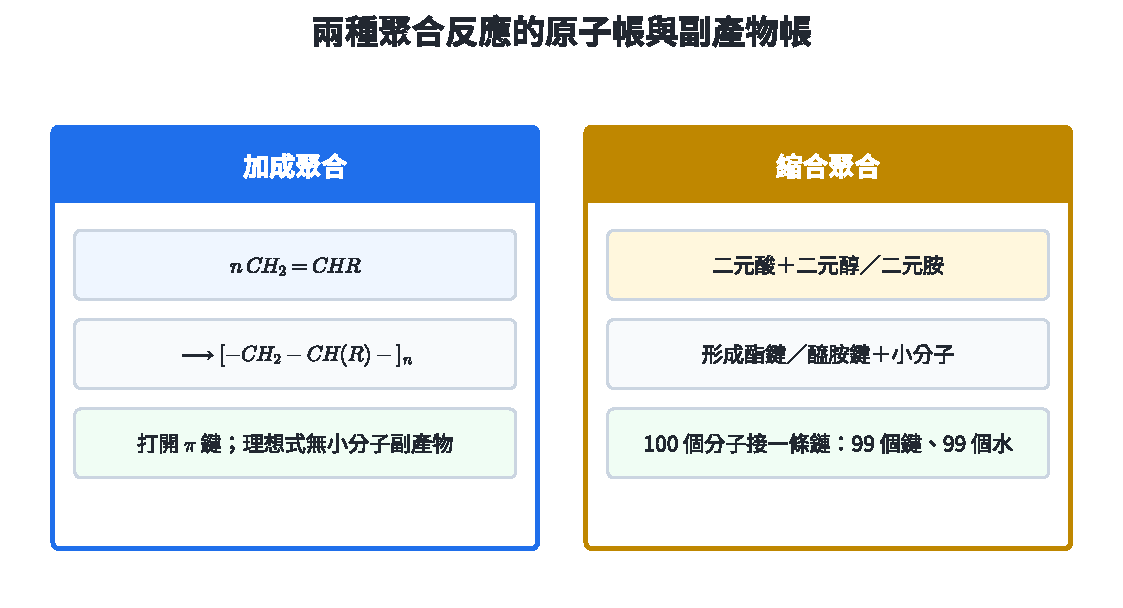
\includegraphics[width=0.99\linewidth,height=\textheight,keepaspectratio,alt={圖 11｜加成聚合保留取代基並打開雙鍵；縮合聚合把雙官能基單體交替相接並產生小分子。}]{assets/選化V-1-加成與縮合聚合.pdf}
\caption{圖 11｜加成聚合保留取代基並打開雙鍵；縮合聚合把雙官能基單體交替相接並產生小分子。}
\end{figure}

\begin{figure}
\centering
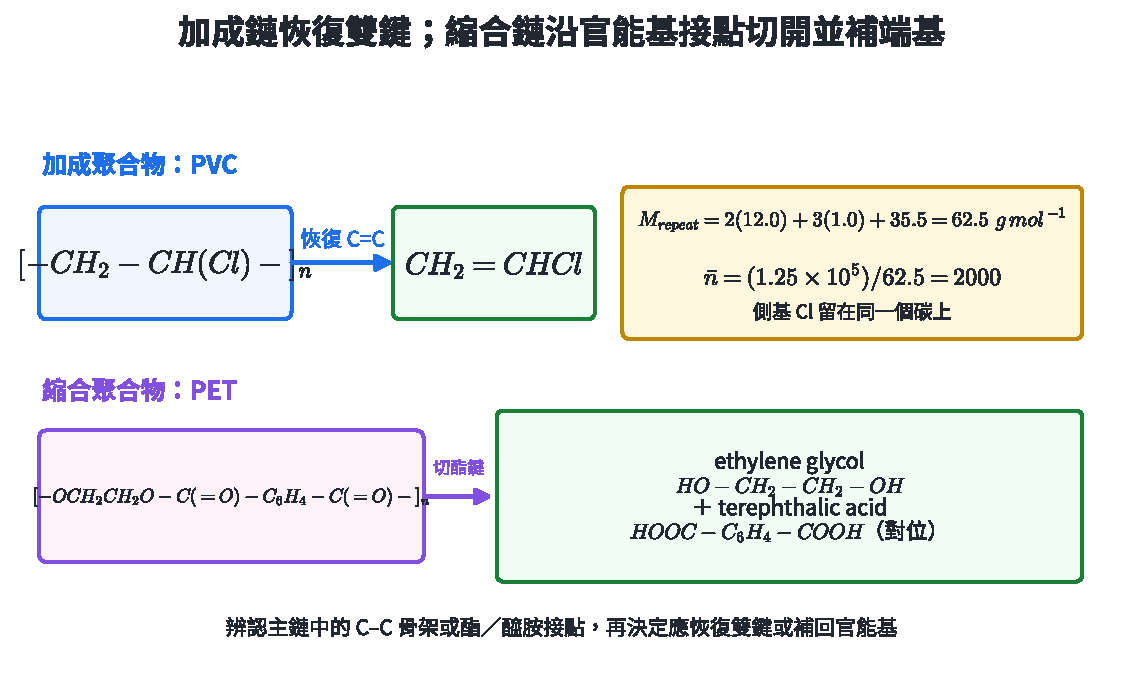
\includegraphics[width=0.98\linewidth,height=\textheight,keepaspectratio,alt={圖 12｜PVC 的兩個主鏈碳間恢復雙鍵可得氯乙烯；PET 沿酯鍵切開並補回端基，可得乙二醇與對苯二甲酸。}]{assets/選化V-1-聚合物反推單體.pdf}
\caption{圖 12｜PVC 的兩個主鏈碳間恢復雙鍵可得氯乙烯；PET 沿酯鍵切開並補回端基，可得乙二醇與對苯二甲酸。}
\end{figure}

\begin{HandoutWorkedExample}

\subsection{示範 13｜由重複單元求單體與聚合度}\label{ux793aux7bc4-13ux7531ux91cdux8907ux55aeux5143ux6c42ux55aeux9ad4ux8207ux805aux5408ux5ea6}

聚合物重複單元為 \([-CH_2-CHCl-]\)，可在兩個主鏈碳之間恢復雙鍵，單體是 vinyl chloride \(CH_2=CHCl\)。重複單元式量為

\[
2(12.0)+3(1.0)+35.5=62.5.
\]

若聚合物平均莫耳質量為 \(1.25\times10^5\ \mathrm{g\,mol^{-1}}\)，

\[
\bar n=\frac{1.25\times10^5}{62.5}=2.00\times10^3.
\]

此值是平均聚合度；實際樣品通常含不同鏈長的分布。

\end{HandoutWorkedExample}

\begin{HandoutWorkedExample}

\subsection{示範 14｜nylon-6,6 的單體與縮合水量}\label{ux793aux7bc4-14nylon-66-ux7684ux55aeux9ad4ux8207ux7e2eux5408ux6c34ux91cf}

nylon-6,6 的重複片段含

\[
[-NH-(CH_2)_6-NH-CO-(CH_2)_4-CO-].
\]

在醯胺鍵 \(-NH-CO-\) 處切開並補回 \(NH_2\) 與 \(COOH\)，得 hexane-1,6-diamine \(H_2N(CH_2)_6NH_2\) 與 hexanedioic acid \(HOOC(CH_2)_4COOH\)。

若各取 100 個分子形成一條交替、兩端保留官能基的線型鏈，起初有 200 個分子，連成一條鏈需 199 次分子間縮合，故放出 199 個 \(H_2O\)。用 \(n\) 個重複單元近似式時常寫 \(2nH_2O\)；精確端基帳需依題目給的鏈端計算。

\end{HandoutWorkedExample}

\subsection{直接用途與適用邊界}\label{ux76f4ux63a5ux7528ux9014ux8207ux9069ux7528ux908aux754c-6}

\begin{itemize}
\tightlist
\item
  由重複單元反推單體可判斷塑膠來源與反應類型，是材料辨識與回收流程的第一層結構資訊。
\item
  聚合度影響黏度、強度與加工；單一平均值無法描述完整分子量分布，工程性質還受支鏈、結晶與添加劑影響。
\item
  縮合副產物的莫耳數需按「實際形成幾個鏈間鍵」計數；無限鏈重複式適合表示骨架，不含完整端基帳。
\end{itemize}

\subsection{練習 7}\label{ux7df4ux7fd2-7}

\begin{enumerate}
\def\labelenumi{\arabic{enumi}.}
\tightlist
\item
  寫出 propene 加成聚合的重複單元，並圈出側鏈。
\item
  某 polyethylene 樣品平均莫耳質量 \(2.80\times10^5\ \mathrm{g\,mol^{-1}}\)，以重複單元 \(C_2H_4\) 求平均聚合度。
\item
  由聚酯片段 \([-OCH_2CH_2OCOC_6H_4CO-]_n\) 反推兩種單體。
\item
  50 個二元醇分子與 50 個二元酸分子完全接成一條線型交替鏈，求形成的酯鍵數與放出的水分子數。
\end{enumerate}

\subsection{練習 7 解析}\label{ux7df4ux7fd2-7-ux89e3ux6790}

\begin{enumerate}
\def\labelenumi{\arabic{enumi}.}
\tightlist
\item
  \(nCH_2=CHCH_3\rightarrow[-CH_2-CH(CH_3)-]_n\)，側鏈是每隔一個主鏈碳所連的 \(CH_3\)。
\item
  \(M(C_2H_4)=28.0\ \mathrm{g\,mol^{-1}}\)，故 \(\bar n=(2.80\times10^5)/28.0=1.00\times10^4\)。
\item
  在酯鍵切開並補 \(OH\) 與 \(COOH\)，得 ethane-1,2-diol \(HOCH_2CH_2OH\) 與 benzene-1,4-dicarboxylic acid \(HOOCC_6H_4COOH\)。
\item
  100 個分子接成一條鏈需 99 個鏈間鍵；每形成一個酯鍵放出一個水，故有 99 個酯鍵並放出 99 個水分子。
\end{enumerate}

\section{8. 天然聚合物}\label{ux5929ux7136ux805aux5408ux7269}

\subsection{8.1 天然橡膠與交聯}\label{ux5929ux7136ux6a61ux81a0ux8207ux4ea4ux806f}

天然橡膠的主要成分是 cis-1,4-polyisoprene，由 isoprene

\[
CH_2=C(CH_3)-CH=CH_2
\]

進行 1,4-加成形成；重複單元仍保留一個 \(C=C\)。cis 組態使鏈呈彎折並較難緊密排列，鏈段可在受力時伸展、卸力後靠熱運動回復。少量硫交聯把不同鏈連成網狀，可降低鏈的永久滑移，改善彈性、耐熱與耐磨。交聯過少時材料易黏軟，交聯過多時鏈段活動受限而變硬。

\subsection{8.2 多醣：鍵結方向改變可消化性與形態}\label{ux591aux91a3ux9375ux7d50ux65b9ux5411ux6539ux8b8aux53efux6d88ux5316ux6027ux8207ux5f62ux614b}

澱粉、肝醣與纖維素都由葡萄糖單元縮合而成，但糖苷鍵方向與支化程度不同：

{\def\LTcaptype{none} % do not increment counter
\begin{longtable}[]{@{}
  >{\raggedright\arraybackslash}p{(\linewidth - 4\tabcolsep) * \real{0.3333}}
  >{\raggedright\arraybackslash}p{(\linewidth - 4\tabcolsep) * \real{0.3333}}
  >{\raggedright\arraybackslash}p{(\linewidth - 4\tabcolsep) * \real{0.3333}}@{}}
\toprule\noalign{}
\begin{minipage}[b]{\linewidth}\raggedright
聚合物
\end{minipage} & \begin{minipage}[b]{\linewidth}\raggedright
主要鍵結與支化
\end{minipage} & \begin{minipage}[b]{\linewidth}\raggedright
結構與功能
\end{minipage} \\
\midrule\noalign{}
\endhead
\bottomrule\noalign{}
\endlastfoot
直鏈澱粉 & \(\alpha(1\rightarrow4)\) & 易形成螺旋；植物儲能 \\
支鏈澱粉 & \(\alpha(1\rightarrow4)\) 主鏈、\(\alpha(1\rightarrow6)\) 分支 & 多個鏈端，較易動員 \\
肝醣 & 同上但分支更密 & 動物快速儲存與釋放葡萄糖 \\
纖維素 & \(\beta(1\rightarrow4)\) & 直鏈間氫鍵形成纖維；植物細胞壁 \\
\end{longtable}
}

人體澱粉酶可催化多數 \(\alpha\) 鍵水解，缺乏分解纖維素 \(\beta(1\rightarrow4)\) 鍵的酵素，因此纖維素主要作膳食纖維。兩者分子式相近，性質差異來自立體鍵結與高階排列。

\subsection{8.3 蛋白質與核酸}\label{ux86cbux767dux8ceaux8207ux6838ux9178}

\(\alpha\)-胺基酸的一般結構為 \(H_2N-CH(R)-COOH\)。兩個胺基酸以胺基與羧基縮合形成\textbf{肽鍵} \(-CO-NH-\) 並放出水；\(n\) 個胺基酸接成一條無環多肽共有 \(n-1\) 個肽鍵並放出 \(n-1\) 個水。胺基酸序列是一次結構，氫鍵、離子作用、疏水作用與二硫鍵等共同建立較高階結構。變性會改變高階結構與功能，通常不等同於肽鍵全部水解。

核苷酸由磷酸、五碳糖與含氮鹼基組成。核苷酸以磷酸二酯鍵連成核酸主鏈；DNA 常為互補雙股，A--T、G--C 的配對以氫鍵穩定，RNA 常為單股且以 U 取代 T。鹼基配對提供資訊複製的結構基礎；共價主鏈維持序列連續。

\begin{figure}
\centering
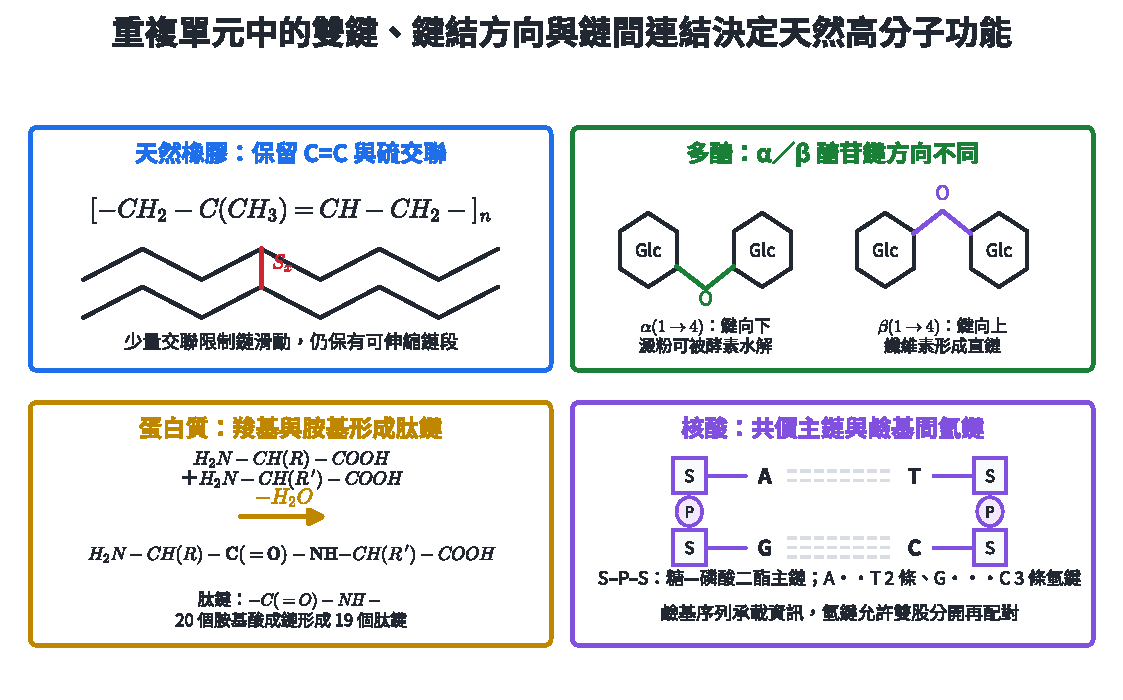
\includegraphics[width=0.99\linewidth,height=\textheight,keepaspectratio,alt={圖 13｜天然橡膠的雙鍵與硫交聯、多醣的 α／β 醣苷鍵、蛋白質的肽鍵及核酸的糖---磷酸主鏈與鹼基氫鍵，分別連到巨觀功能。}]{assets/選化V-1-天然聚合物鍵結.pdf}
\caption{圖 13｜天然橡膠的雙鍵與硫交聯、多醣的 α／β 醣苷鍵、蛋白質的肽鍵及核酸的糖---磷酸主鏈與鹼基氫鍵，分別連到巨觀功能。}
\end{figure}

\begin{HandoutWorkedExample}

\subsection{示範 15｜由多醣資料判斷澱粉或纖維素}\label{ux793aux7bc4-15ux7531ux591aux91a3ux8cc7ux6599ux5224ux65b7ux6fb1ux7c89ux6216ux7e96ux7dadux7d20}

樣品 X 與 Y 的元素組成相近。X 遇碘呈藍黑色，可被澱粉酶逐步水解成較小糖；Y 形成高抗拉纖維，澱粉酶處理後質量幾乎不變。

X 的碘呈色與酵素水解共同支持澱粉，其主鏈為 \(\alpha(1\rightarrow4)\)；Y 的纖維性與對澱粉酶穩定共同支持纖維素，其主鏈為 \(\beta(1\rightarrow4)\)。兩者的關鍵差異在糖苷鍵立體方向與鏈間排列，需用結構或反應證據補足相近的元素組成。

\end{HandoutWorkedExample}

\begin{HandoutWorkedExample}

\subsection{示範 16｜多肽縮合的質量帳}\label{ux793aux7bc4-16ux591aux80bdux7e2eux5408ux7684ux8ceaux91cfux5e33}

由 20 個 glycine（\(M=75.0\ \mathrm{g\,mol^{-1}}\)）形成一條無環多肽。需形成 \(20-1=19\) 個肽鍵，放出 19 個水：

\[
M(\text{多肽})=20(75.0)-19(18.0)=1158\ \mathrm{g\,mol^{-1}}.
\]

若題目改成形成兩條各含 10 個單元的鏈，肽鍵總數為 \(2(10-1)=18\)，會比單一 20-mer 少放一個水；水量取決於鏈數與成鍵數。

\end{HandoutWorkedExample}

\subsection{直接用途與適用邊界}\label{ux76f4ux63a5ux7528ux9014ux8207ux9069ux7528ux908aux754c-7}

\begin{itemize}
\tightlist
\item
  硫化調整輪胎與橡膠零件的交聯密度；最佳性能需在彈性、硬度與加工間取得合適交聯範圍。
\item
  糖苷鍵方向解釋食物澱粉可供能而纖維素作纖維；實際消化還受顆粒結構、加熱與腸道微生物影響。
\item
  蛋白質序列與折疊用於酵素、抗體與食品加工；由序列預測完整功能仍需環境與三維結構資料。
\item
  DNA 互補配對用於聚合酶連鎖反應與序列檢測；配對規則說明選擇性，實際穩定度還受序列、鹽度與溫度影響。
\end{itemize}

\subsection{練習 8}\label{ux7df4ux7fd2-8}

\begin{enumerate}
\def\labelenumi{\arabic{enumi}.}
\tightlist
\item
  寫出 isoprene 的分子式，並指出天然橡膠重複單元中保留幾個雙鍵。
\item
  比較肝醣與直鏈澱粉的分支程度，說明分支如何影響酵素可同時作用的鏈端數。
\item
  由 12 個胺基酸形成一條無環多肽，求肽鍵數與放出的水分子數；若分成兩條各 6 個單元，重新計算。
\item
  一段 DNA 單股序列為 5′-AGCTAC-3′。寫出互補股序列及方向，並計算此雙股片段的 A--T 與 G--C 鹼基對數。
\end{enumerate}

\subsection{練習 8 解析}\label{ux7df4ux7fd2-8-ux89e3ux6790}

\begin{enumerate}
\def\labelenumi{\arabic{enumi}.}
\tightlist
\item
  isoprene 為 \(C_5H_8\)。1,4-加成消耗共軛雙鍵中的一部分，每個天然橡膠重複單元保留一個 \(C=C\)。
\item
  肝醣分支遠多於直鏈澱粉；每個分支帶來新的非還原端，使多個酵素可同時從不同鏈端釋放葡萄糖單元。
\item
  一條 12-mer 有 \(12-1=11\) 個肽鍵並放 11 個水。兩條 6-mer 各有 5 個，總共 10 個肽鍵並放 10 個水。
\item
  互補反向平行股為 3′-TCGATG-5′。原股有 A 2 個、T 1 個，故 A--T 對 3 組；G 1 個、C 2 個，故 G--C 對 3 組。
\end{enumerate}

\section{9. 人造聚合物}\label{ux4ebaux9020ux805aux5408ux7269}

\subsection{9.1 塑膠、纖維與合成橡膠}\label{ux5851ux81a0ux7e96ux7dadux8207ux5408ux6210ux6a61ux81a0}

人造聚合物的分類反映主要用途，但同一聚合物可跨類別：

{\def\LTcaptype{none} % do not increment counter
\begin{longtable}[]{@{}
  >{\raggedright\arraybackslash}p{(\linewidth - 4\tabcolsep) * \real{0.3333}}
  >{\raggedright\arraybackslash}p{(\linewidth - 4\tabcolsep) * \real{0.3333}}
  >{\raggedright\arraybackslash}p{(\linewidth - 4\tabcolsep) * \real{0.3333}}@{}}
\toprule\noalign{}
\begin{minipage}[b]{\linewidth}\raggedright
材料
\end{minipage} & \begin{minipage}[b]{\linewidth}\raggedright
重複結構或關鍵作用
\end{minipage} & \begin{minipage}[b]{\linewidth}\raggedright
性質與用途
\end{minipage} \\
\midrule\noalign{}
\endhead
\bottomrule\noalign{}
\endlastfoot
PE & 非極性 \(-CH_2-CH_2-\) & 防水、電絕緣、包裝 \\
PP & 每兩碳一個 \(CH_3\) 側基 & 較硬、耐疲勞，容器與鉸鏈 \\
PVC & 每兩碳一個 Cl & 極性、阻燃性較佳，管材與線皮；性質強受增塑劑影響 \\
PS & 苯基側鏈 & 硬而較脆；發泡後隔熱 \\
PMMA & 大型極性酯側基 & 透明、耐候，光學板材 \\
PET & 芳香族聚酯主鏈 & 強度、阻氣性與纖維形成性佳 \\
nylon-6,6 & 聚醯胺主鏈 & 氫鍵、耐磨，工程塑膠與纖維 \\
SBR／NBR & 共聚合成橡膠 & 前者耐磨；後者極性腈基提高耐油性 \\
silicone & \(-Si-O-\) 主鏈 & 柔韌、耐候、耐溫範圍寬 \\
\end{longtable}
}

纖維需要鏈能沿拉伸方向排列並形成足夠鏈間作用力；彈性體需要柔軟鏈段與少量交聯；硬質塑膠則可由剛性骨架、結晶或較高交聯限制鏈段運動。

\subsection{9.2 熱塑性、熱固性與材料循環}\label{ux71b1ux5851ux6027ux71b1ux56faux6027ux8207ux6750ux6599ux5faaux74b0}

\textbf{熱塑性聚合物}主要由線型或支鏈構成，加熱使鏈段可相對移動，能再熔融加工。\textbf{熱固性聚合物}形成高度交聯網狀結構，受熱時無法靠整條鏈流動，強熱下通常分解。彈性體常介於兩者之間，以低密度交聯兼顧形變與回復。

回收路徑需配合結構：

\begin{itemize}
\tightlist
\item
  機械回收：分選、清洗、熔融再造粒，適合污染少且可再熔融的熱塑性塑膠；熱歷史會使鏈劣化。
\item
  化學回收：將聚酯、聚醯胺等裂解為單體或較小分子，能處理部分品質下降材料，但需能量與純化。
\item
  能量回收：燃燒取得能量，需控制 CO、粒狀物、酸性氣體與其他排放；保留的材料價值最低。
\item
  源頭減量與重複使用：直接減少新聚合物與廢棄物生成，通常早於末端回收考量。
\end{itemize}

材料標示碼提供樹脂類別線索，並不等同於當地一定可回收；顏料、填料、多層複合與食物污染都影響實際流程。

\begin{figure}
\centering
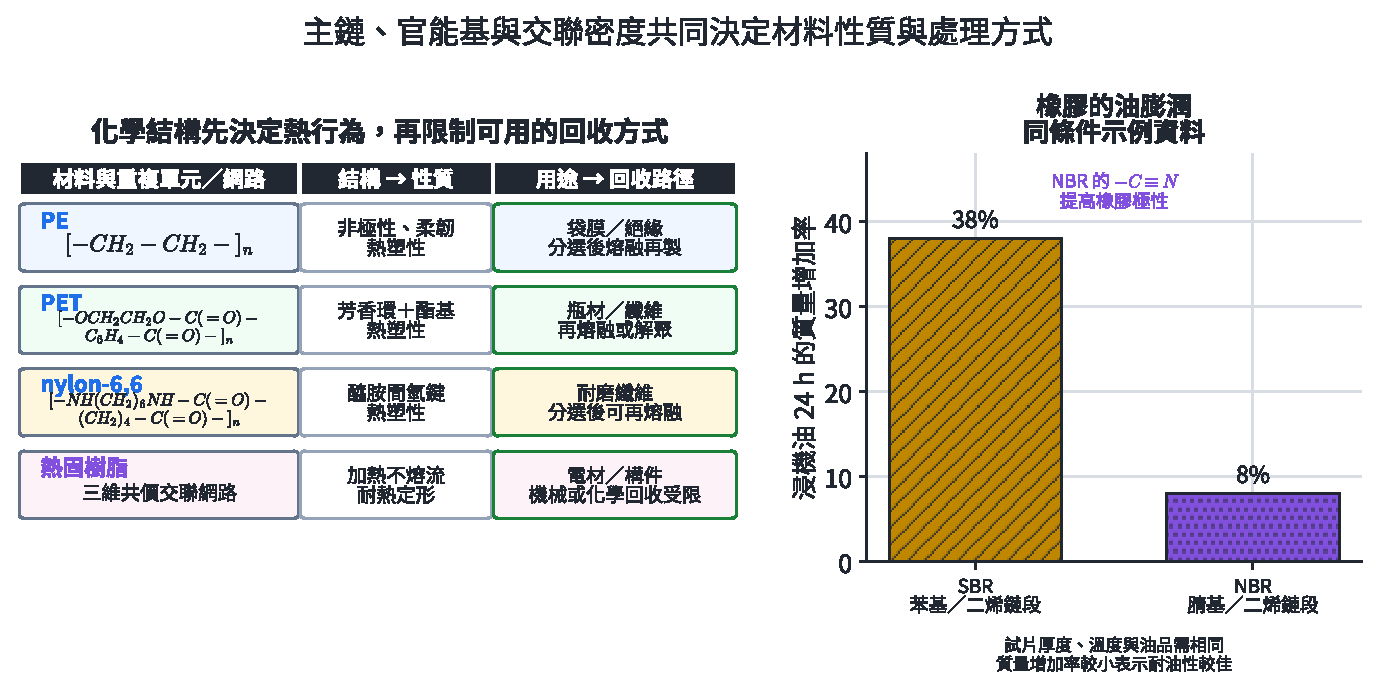
\includegraphics[width=0.99\linewidth,height=\textheight,keepaspectratio,alt={圖 14｜PE、PET、nylon-6,6 與熱固樹脂的重複單元或網路連到熱行為與回收路徑；SBR／NBR 的同條件資料示範官能基如何影響油膨潤。}]{assets/選化V-1-人造聚合物結構與用途.pdf}
\caption{圖 14｜PE、PET、nylon-6,6 與熱固樹脂的重複單元或網路連到熱行為與回收路徑；SBR／NBR 的同條件資料示範官能基如何影響油膨潤。}
\end{figure}

\begin{HandoutWorkedExample}

\subsection{示範 17｜由結構選擇飲料瓶與袋膜材料}\label{ux793aux7bc4-17ux7531ux7d50ux69cbux9078ux64c7ux98f2ux6599ux74f6ux8207ux888bux819cux6750ux6599}

情境 A 需透明、較佳阻氣性並能製成硬瓶；情境 B 需柔軟、防水且成本低的薄膜。PET 主鏈含芳香環與酯基，骨架較剛且鏈間作用較強，適合 A。低密度 PE 為非極性柔軟鏈且支鏈妨礙緊密結晶，適合 B。

兩者都是熱塑性聚合物，可再熔融；實際回收仍需分流，因混合不同聚合物會使熔融加工與機械性質不穩定。

\end{HandoutWorkedExample}

\begin{HandoutWorkedExample}

\subsection{示範 18｜由資料選擇耐油彈性體}\label{ux793aux7bc4-18ux7531ux8cc7ux6599ux9078ux64c7ux8010ux6cb9ux5f48ux6027ux9ad4}

兩種橡膠浸在非極性機油 24 h：SBR 質量增加 38\%，NBR 質量增加 8\%；兩者拉伸回復率相近。NBR 含極性 \(-C\equiv N\) 側基，使其與非極性油的相容性較低，吸油膨潤較小，因此應選 NBR 作油封。

若應用改為低溫輪胎胎面，還需比較玻璃轉移溫度、磨耗與濕地抓地；單一吸油數據只支持耐油性選擇。

\end{HandoutWorkedExample}

\subsection{直接用途與適用邊界}\label{ux76f4ux63a5ux7528ux9014ux8207ux9069ux7528ux908aux754c-8}

\begin{itemize}
\tightlist
\item
  包裝、纖維、線纜與密封件的材料選擇可由主鏈剛性、側基極性、氫鍵與交聯建立第一層預測，再用實測規格確認。
\item
  熱塑／熱固分類直接決定熔融加工與機械回收可能性；添加劑與複合結構可能改變實際行為。
\item
  生物可分解、可堆肥與可回收是不同條件；標示需連到溫度、濕度、微生物與處理設施，才可判斷環境結果。
\end{itemize}

\subsection{練習 9}\label{ux7df4ux7fd2-9}

\begin{enumerate}
\def\labelenumi{\arabic{enumi}.}
\tightlist
\item
  由重複單元 \([-CH_2-C(CH_3)_2-]_n\) 反推單體，並判斷屬加成或縮合聚合。
\item
  比較 nylon-6,6 與 PE 的鏈間作用力，預測哪一種較適合耐磨纖維並說明。
\item
  一個聚合物加熱可軟化重塑，另一個維持形狀至高溫後焦化。以鏈結構分類兩者，並提出對應回收路徑。
\item
  某密封材料在水、機油中的質量增加率如下：材料 P 為 2\%、35\%；材料 Q 為 5\%、7\%。若需接觸機油且保持尺寸，選哪一種？說明數據能支持與尚未支持的結論。
\end{enumerate}

\subsection{練習 9 解析}\label{ux7df4ux7fd2-9-ux89e3ux6790}

\begin{enumerate}
\def\labelenumi{\arabic{enumi}.}
\tightlist
\item
  在兩主鏈碳間恢復雙鍵得 \(CH_2=C(CH_3)_2\)（2-methylpropene）；過程開啟雙鍵且無小分子副產物，屬加成聚合。
\item
  nylon-6,6 的醯胺基可形成鏈間氫鍵，PE 主要為分散力；在其他條件相近時 nylon-6,6 較能抵抗鏈滑移，適合耐磨纖維。
\item
  可軟化重塑者為線型或支鏈的熱塑性聚合物，可分選後機械回收；高溫不流動而焦化者是高度交聯熱固性聚合物，較適合化學回收、粉碎作填料或受控能量回收。
\item
  選 Q，因在機油中的質量增加僅 7\%，膨潤遠小於 P 的 35\%。資料支持耐油尺寸穩定性的相對比較；尚未測得抗拉、溫度範圍、老化與密封壽命。
\end{enumerate}

\section{10. 核心整理}\label{ux6838ux5fc3ux6574ux7406}

{\def\LTcaptype{none} % do not increment counter
\begin{longtable}[]{@{}
  >{\raggedright\arraybackslash}p{(\linewidth - 4\tabcolsep) * \real{0.3333}}
  >{\raggedright\arraybackslash}p{(\linewidth - 4\tabcolsep) * \real{0.3333}}
  >{\raggedright\arraybackslash}p{(\linewidth - 4\tabcolsep) * \real{0.3333}}@{}}
\toprule\noalign{}
\begin{minipage}[b]{\linewidth}\raggedright
結構資訊
\end{minipage} & \begin{minipage}[b]{\linewidth}\raggedright
可推出的第一層結論
\end{minipage} & \begin{minipage}[b]{\linewidth}\raggedright
還需要的證據
\end{minipage} \\
\midrule\noalign{}
\endhead
\bottomrule\noalign{}
\endlastfoot
分子式與 DBE & 環與多重鍵的總約束 & 官能基檢驗、光譜或物性才可定結構 \\
官能基 & 典型極性、酸鹼與反應位置 & 試劑條件、對照組與交叉檢驗 \\
羥基碳的取代數 & 一級醇→醛→酸；二級醇→酮 & 氧化劑強度與產物分析 \\
\(C=C\)／\(C\equiv C\) & 可發生加成，常使溴水或 \(KMnO_4\) 褪色 & 其他還原性物質也可造成褪色 \\
\(-CHO\)／\(-CO-\) & 醛較易呈銀鏡；酮通常無此反應 & 已知陽性對照與空白組 \\
\(-COOH\)／\(-NH_2\) & 可用酸鹼轉成水溶性離子 & pH、溶劑互不相溶與層位資料 \\
聚合物重複單元 & 可反推單體與聚合類型 & 端基、分子量分布、支鏈與交聯 \\
鍵結方向、分支、交聯 & 可解釋消化、彈性、流動與回收 & 溫度、添加劑與實測材料規格 \\
\end{longtable}
}

反應路線的共同檢查順序為：

\begin{enumerate}
\def\labelenumi{\arabic{enumi}.}
\tightlist
\item
  守恆碳骨架與各元素原子數。
\item
  標出實際改變的官能基與斷鍵、成鍵位置。
\item
  把試劑與溫度寫在箭頭上，使產物選擇有條件。
\item
  將「觀察到的顏色、氣體、沉澱、熔點或層位」和「推論出的官能基或純度」分開。
\item
  定量題再檢查限量、係數、單位、端基或鏈數。
\end{enumerate}

\section{11. 章末分層題}\label{ux7ae0ux672bux5206ux5c64ux984c}

\subsection{基礎與模型題 1--4}\label{ux57faux790eux8207ux6a21ux578bux984c-14}

\begin{enumerate}
\def\labelenumi{\arabic{enumi}.}
\tightlist
\item
  分子式 \(C_5H_{10}O_2\) 的 DBE 為何？若已知它是非環狀飽和單羧酸，DBE 由哪個鍵結提供？寫出一個直鏈結構與一個支鏈結構。
\item
  \(0.740\ \mathrm g\) 的 C、H、O 化合物完全燃燒，得 \(1.32\ \mathrm g\ CO_2\) 與 \(0.540\ \mathrm g\ H_2O\)。分子量為 \(74.0\)，求實驗式與分子式。
\item
  命名 \(CH_3CH=C(CH_3)CH_2OH\)，並說明主鏈編號方向。
\item
  1 mol buta-1,3-diene 含兩個 \(C=C\)。求完全加成最多可消耗的 \(H_2\) 與 \(Br_2\) 莫耳數，並寫出完全氫化產物。
\end{enumerate}

\subsection{官能基與分離題 5--7}\label{ux5b98ux80fdux57faux8207ux5206ux96e2ux984c-57}

\begin{enumerate}
\def\labelenumi{\arabic{enumi}.}
\setcounter{enumi}{4}
\tightlist
\item
  A、B、C 都是 \(C_4H_{10}O\) 異構物。A 氧化後呈銀鏡；B 氧化後生成不呈銀鏡的羰基化合物；C 沸點顯著較低且溫和氧化無反應。各寫出一個可能結構並分類。
\item
  ethyl methanoate 在酸性水解與鹼性水解中的含碳產物各為何？指出哪一組條件形成羧酸鹽。
\item
  乙醚層含 benzoic acid、aniline 與 naphthalene。請依序設計酸鹼萃取，把三者分開並回收到中性物質；寫出兩個成鹽／復原反應。
\end{enumerate}

\subsection{聚合物與生物分子題 8--11}\label{ux805aux5408ux7269ux8207ux751fux7269ux5206ux5b50ux984c-811}

\begin{enumerate}
\def\labelenumi{\arabic{enumi}.}
\setcounter{enumi}{7}
\tightlist
\item
  某加成聚合物的重複單元為 \([-CH_2-CH(CN)-]_n\)，平均莫耳質量為 \(5.30\times10^4\ \mathrm{g\,mol^{-1}}\)。反推單體，並以重複單元式量 \(53.0\) 求平均聚合度。
\item
  兩種多醣 U、V 都由 glucose 單元組成。U 具 \(\alpha(1\rightarrow4)\) 主鏈與密集 \(\alpha(1\rightarrow6)\) 分支；V 為 \(\beta(1\rightarrow4)\) 直鏈並形成纖維。判斷 U、V，並比較人體酵素可利用性。
\item
  由 8 個胺基酸形成一條直鏈多肽時，形成幾個肽鍵並放出幾個水？若其中一段 DNA 雙股含 40 個鹼基對，其中 14 對為 G--C，求 A--T 對數與整段氫鍵總數。
\item
  某透明容器材料的主鏈含芳香環與酯基，可再熔融；某鍋具把手為高度交聯網狀，受熱不軟化流動。分別判斷較可能是熱塑性聚酯或熱固性樹脂，並提出適合的材料處理路徑。
\end{enumerate}

\subsection{實驗題 12}\label{ux5be6ux9a57ux984c-12}

\begin{enumerate}
\def\labelenumi{\arabic{enumi}.}
\setcounter{enumi}{11}
\tightlist
\item
  水楊酸與阿司匹靈樣品分別加入 \(FeCl_3\)：前者深紫、後者極淡。另測得阿司匹靈樣品熔點 \(134\)--\(136^\circ\mathrm C\)。分別寫出呈色與熔點資料支持的結論，並指出每項資料仍需的對照。
\end{enumerate}

\subsection{跨節整合題 13--16}\label{ux8de8ux7bc0ux6574ux5408ux984c-1316}

\begin{enumerate}
\def\labelenumi{\arabic{enumi}.}
\setcounter{enumi}{12}
\tightlist
\item
  未知含氧化合物 X 只含 C、H、O。\(0.580\ \mathrm g\) X 完全燃燒得 \(1.32\ \mathrm g\ CO_2\) 與 \(0.540\ \mathrm g\ H_2O\)，分子量為 \(58.0\)。X 呈銀鏡；溫和氧化後的 Y 可與 \(NaHCO_3\) 放出 \(CO_2\)。求 X 的分子式、DBE、結構與 Y，並寫出證據鏈。
\item
  一份乙醚溶液含 aniline、benzoic acid 與 naphthalene。操作甲加入稀 HCl；操作乙對分出的有機層加入 \(NaHCO_3\)。請畫出每步水層／有機層的主要物種，寫出回收三種中性物質的方法，並說明為何操作乙伴隨洩壓。
\item
  PET 由 ethane-1,2-diol 與 benzene-1,4-dicarboxylic acid 縮合。各取 50 個分子接成一條交替線型鏈：（a）形成幾個酯鍵並放出幾個水？（b）若 PET 重複單元式量為 \(192\)、平均莫耳質量 \(3.84\times10^4\ \mathrm{g\,mol^{-1}}\)，求平均聚合度。（c）比較 PET 與硫化天然橡膠的鏈結構，解釋前者適合作纖維／瓶材、後者適合作彈性體。
\item
  以 \(2.76\ \mathrm g\) 水楊酸（\(M=138\)）和過量醋酸酐製備阿司匹靈（\(M=180\)）。未充分乾燥的粗晶質量 \(3.78\ \mathrm g\)；再結晶、乾燥後得 \(2.88\ \mathrm g\)，\(FeCl_3\) 只呈極淡紫色，熔點 \(134\)--\(136^\circ\mathrm C\)。（a）求理論質量、粗晶表觀產率與乾燥純化後產率。（b）解釋粗晶超過 \(100\%\) 的原因。（c）評估純化後的純度證據。（d）提出一個空白或對照、兩項關鍵安全措施與廢液分類。
\end{enumerate}

\section{12. 章末分層題詳解}\label{ux7ae0ux672bux5206ux5c64ux984cux8a73ux89e3}

\subsection{第 1 題}\label{ux7b2c-1-ux984c}

\[
\mathrm{DBE}=\frac{2(5)+2-10}{2}=1.
\]

非環狀飽和單羧酸不含碳---碳多重鍵，因此唯一 DBE 由羧基的 \(C=O\) 提供。直鏈可寫 pentanoic acid：\(CH_3CH_2CH_2CH_2COOH\)；支鏈可寫 3-methylbutanoic acid：\(CH_3CH(CH_3)CH_2COOH\)。兩者均為 \(C_5H_{10}O_2\)，且都只有一個羰基雙鍵。

\subsection{第 2 題}\label{ux7b2c-2-ux984c}

\[
n(C)=n(CO_2)=\frac{1.32}{44.0}=0.0300\ \mathrm{mol},
\]

\[
n(H)=2n(H_2O)=2\left(\frac{0.540}{18.0}\right)=0.0600\ \mathrm{mol}.
\]

C、H 質量分別為 \(0.360\) g、\(0.0600\) g，故

\[
m(O)=0.740-0.360-0.0600=0.320\ \mathrm g,\qquad
n(O)=\frac{0.320}{16.0}=0.0200\ \mathrm{mol}.
\]

原子比 \(0.0300:0.0600:0.0200=3:6:2\)，實驗式 \(C_3H_6O_2\)，式量為 \(74.0\)，與分子量相同，所以分子式也是 \(C_3H_6O_2\)。質量與原子數均閉合。

\subsection{第 3 題}\label{ux7b2c-3-ux984c}

主官能基是醇，選取含 \(OH\) 與 \(C=C\) 的四碳主鏈。由 \(OH\) 端編號使羥基碳為 1，雙鍵位於 2，甲基也位於 2，名稱為 \textbf{2-methylbut-2-en-1-ol（2-甲基-2-丁烯-1-醇）}。若從另一端編號，羥基位碼會變大，與主官能基優先原則不合。

\subsection{第 4 題}\label{ux7b2c-4-ux984c}

buta-1,3-diene 每個分子有兩個 \(C=C\)，每個雙鍵完全加成可消耗 1 mol \(H_2\) 或 1 mol \(Br_2\)，所以 1 mol 分子最多消耗 2 mol \(H_2\) 或 2 mol \(Br_2\)。完全氫化後所有雙鍵成單鍵，產物為 butane：\(CH_3CH_2CH_2CH_3\)。

\subsection{第 5 題}\label{ux7b2c-5-ux984c}

一組符合資料的答案為：

\begin{itemize}
\tightlist
\item
  A：butan-1-ol，屬一級醇；氧化先生成 butanal，呈銀鏡。
\item
  B：butan-2-ol，屬二級醇；氧化生成 butan-2-one，無銀鏡。
\item
  C：ethoxyethane，屬醚；無分子間 \(O-H\) 氫鍵，沸點低於同分子式的醇，且不沿醇的溫和氧化路徑。
\end{itemize}

A 也可選另一個能生成醛的一級醇異構物；答案需同時符合分子式、氧化產物與物性。

\subsection{第 6 題}\label{ux7b2c-6-ux984c}

ethyl methanoate 為 \(HCOOCH_2CH_3\)。

酸性水解：

\[
HCOOCH_2CH_3+H_2O\rightleftharpoons HCOOH+CH_3CH_2OH.
\]

含碳產物為 methanoic acid 與 ethanol。鹼性水解：

\[
HCOOCH_2CH_3+OH^-\rightarrow HCOO^-+CH_3CH_2OH.
\]

含碳產物為 methanoate 與 ethanol；羧酸鹽出現在鹼性條件。兩式均守恆兩個碳。

\subsection{第 7 題}\label{ux7b2c-7-ux984c}

先加稀 HCl，aniline 被質子化成 \(C_6H_5NH_3^+Cl^-\) 進入水層；分出水層，加 \(NaOH\) 復原中性 aniline，再以有機溶劑萃取或分離：

\[
C_6H_5NH_3^++OH^-\rightarrow C_6H_5NH_2+H_2O.
\]

原有機層含 benzoic acid 與 naphthalene。加入 \(NaHCO_3\)：

\[
C_6H_5COOH+HCO_3^-\rightarrow C_6H_5COO^-+CO_2+H_2O.
\]

benzoate 進水層，naphthalene 留有機層，除去乙醚可回收 naphthalene。benzoate 水層加酸至酸性，\(C_6H_5COOH\) 析出並過濾。每次分層先由密度或滴水測試確認層位。

\subsection{第 8 題}\label{ux7b2c-8-ux984c}

在重複單元兩主鏈碳間恢復雙鍵，單體為 acrylonitrile：

\[
CH_2=CHCN.
\]

\[
\bar n=\frac{5.30\times10^4}{53.0}=1.00\times10^3.
\]

這是平均聚合度；由雙鍵開啟、理想化不放出小分子，屬加成聚合。

\subsection{第 9 題}\label{ux7b2c-9-ux984c}

U 具密集 \(\alpha(1\rightarrow6)\) 分支，是肝醣；V 具 \(\beta(1\rightarrow4)\) 直鏈並形成纖維，是纖維素。人體酵素可水解肝醣的 \(\alpha\) 糖苷鍵，且分支提供多個鏈端；人體缺乏纖維素酶，V 主要作膳食纖維。兩者以相同單體形成，性質差異來自鍵結立體方向與分支。

\subsection{第 10 題}\label{ux7b2c-10-ux984c}

8 個胺基酸接成一條直鏈需 \(8-1=7\) 次縮合，所以形成 7 個肽鍵並放出 7 個水。DNA 中

\[
N(A\!-\!T)=40-14=26.
\]

A--T 每對有 2 個氫鍵，G--C 每對有 3 個：

\[
N(\text{氫鍵})=26(2)+14(3)=94.
\]

答案以 40 個鹼基對而非 80 個單一鹼基作總數基準。

\subsection{第 11 題}\label{ux7b2c-11-ux984c}

含芳香環與酯基且可再熔融的容器材料符合 PET 等線型\textbf{熱塑性聚酯}；可分選、清洗後機械回收，也可水解或醇解作化學回收。鍋具把手受熱不流動，符合高度交聯的\textbf{熱固性樹脂}；無法靠熔融重塑，可粉碎作填料、採特定化學回收或受控能量回收。材料處理還需考慮添加劑與污染。

\subsection{第 12 題}\label{ux7b2c-12-ux984c}

水楊酸的酚性 \(OH\) 與 \(Fe^{3+}\) 形成紫色配合物；阿司匹靈樣品極淡呈色支持未反應水楊酸很少。需以純溶劑空白、已知水楊酸陽性對照及已知純阿司匹靈對照確認試劑與背景色。

\(134\)--\(136^\circ\mathrm C\) 的窄熔點區間支持樣品較純，因雜質通常使熔點下降並展寬；仍需與同裝置、同升溫速率測得的標準品或可靠參考區間比較。兩項資料互補：呈色鎖定酚性雜質，熔點反映整體純度。

\subsection{第 13 題｜跨節整合}\label{ux7b2c-13-ux984cux8de8ux7bc0ux6574ux5408}

先做組成帳：

\[
n(C)=\frac{1.32}{44.0}=0.0300\ \mathrm{mol},\qquad
n(H)=2\left(\frac{0.540}{18.0}\right)=0.0600\ \mathrm{mol}.
\]

C、H 質量為 \(0.360+0.0600=0.420\) g，故 O 質量 \(0.160\) g、\(n(O)=0.0100\) mol。原子比為 \(3:6:1\)，實驗式 \(C_3H_6O\)，式量 \(58.0\)，所以分子式亦為 \(C_3H_6O\)。

\[
\mathrm{DBE}=\frac{2(3)+2-6}{2}=1.
\]

銀鏡表示 X 具有可被溫和氧化的醛基；\(C_3H_6O\) 的相應直鏈醛是 propanal \(CH_3CH_2CHO\)，其羰基提供一個 DBE。氧化保持三碳骨架並得 propanoic acid：

\[
CH_3CH_2CHO+[O]\rightarrow CH_3CH_2COOH.
\]

Y 與 \(NaHCO_3\) 放 \(CO_2\)，再支持其為羧酸。證據鏈是「燃燒與分子量定分子式 → DBE 限定一個環／雙鍵單位 → 銀鏡定位醛 → 氧化產物放氣定位羧酸」。

\subsection{第 14 題｜跨節整合}\label{ux7b2c-14-ux984cux8de8ux7bc0ux6574ux5408}

操作甲後：

\begin{itemize}
\tightlist
\item
  水層：\(C_6H_5NH_3^+Cl^-\)。
\item
  有機層：\(C_6H_5COOH\) 與 naphthalene。
\end{itemize}

水層以 \(NaOH\) 調成鹼性，使 \(C_6H_5NH_3^+\) 去質子化成 aniline，再萃取或分離中性 aniline。

操作乙後：

\begin{itemize}
\tightlist
\item
  水層：\(C_6H_5COO^-\) 與水相陽離子，並生成 \(CO_2\)。
\item
  有機層：naphthalene。
\end{itemize}

對 benzoate 水層加 HCl，生成中性 benzoic acid 沉澱；有機層除去乙醚回收 naphthalene。操作乙會放出 \(CO_2\)，密閉分液漏斗內壓上升，故每次輕搖後都要朝無人方向洩壓。這項提醒會直接影響操作安全。

\subsection{第 15 題｜跨節整合}\label{ux7b2c-15-ux984cux8de8ux7bc0ux6574ux5408}

（a）50 個二元醇與 50 個二元酸共有 100 個分子；接成一條線型鏈需 99 個分子間連接。每個連接形成一個酯鍵並放出一個水，所以形成 99 個酯鍵、放出 99 個 \(H_2O\)。端基各保留一個官能基。

（b）

\[
\bar n=\frac{3.84\times10^4}{192}=200.
\]

（c）PET 主鏈含芳香環與酯基，骨架較剛、鏈間偶極作用較強，線型鏈可排列並拉伸定向，所以適合作強韌纖維與阻氣瓶材。天然橡膠的 cis-polyisoprene 主鏈彎曲且鏈段柔軟；少量硫交聯防止永久滑移，受力伸展後可回復，因此適合作彈性體。若把橡膠交聯密度大幅提高，鏈段活動減少，材料會變硬。

\subsection{第 16 題｜跨節整合}\label{ux7b2c-16-ux984cux8de8ux7bc0ux6574ux5408}

（a）水楊酸為限量：

\[
n=\frac{2.76}{138}=0.0200\ \mathrm{mol},
\qquad
m_{\mathrm{theory}}=0.0200(180)=3.60\ \mathrm g.
\]

粗晶表觀產率：

\[
\frac{3.78}{3.60}\times100\%=105\%.
\]

乾燥純化後產率：

\[
\frac{2.88}{3.60}\times100\%=80.0\%.
\]

（b）表觀產率超過 \(100\%\) 表示秤得物不全是乾燥阿司匹靈，可能夾帶母液、水、醋酸、水楊酸或其他雜質；它不表示生成量超過限量反應物允許的理論值。

（c）\(FeCl_3\) 僅極淡紫色支持酚性水楊酸殘留少；\(134\)--\(136^\circ\mathrm C\) 的窄區間支持純度較高。兩者仍應與水楊酸陽性對照、純阿司匹靈對照及相同裝置的熔點標準比較，才能排除試劑失效或量測偏差。

（d）可設「同體積溶劑＋\(FeCl_3\)」空白，以及已知水楊酸、已知純阿司匹靈對照。關鍵安全措施包括在通風櫥處理醋酸酐與濃酸、全程戴護目鏡及適用手套，且減壓過濾前檢查玻璃器材。含有機物母液收入有機廢液，酸性水相依酸性含有機物廢液規定收集，固體殘渣另收。


\end{document}
